\documentclass{article}

\usepackage{amsmath,geometry,amsfonts,array,makecell,enumitem,bm,esint,booktabs,multirow,mathtools,upgreek,amssymb,pgfplots,mathrsfs,nicematrix,slashed, chemfig, tikzorbital}
\usepackage[amsmath]{ntheorem}
\usepackage[hidelinks,naturalnames]{hyperref}
\usepackage[nameinlink,noabbrev]{cleveref}
\usepackage{fancyhdr}
\pagestyle{fancy}
\fancyhead[L]{\itshape\nouppercase{\leftmark}}
\fancyhead[R]{M1 Inorganic Materials}

\title{Inorganic Materials}
\author{Yue Wu}

\geometry{a4paper,hmargin=1.1in,vmargin=1.2in}

\setlength{\parskip}{1em}
\tolerance=1000
\emergencystretch=1em
\hyphenpenalty=1000
\exhyphenpenalty=100
\righthyphenmin=3

\pgfplotsset{compat=1.18}
\usetikzlibrary{decorations.markings}

\theoremstyle{plain}\theoremheaderfont{\normalfont\itshape}\theorembodyfont{\rmfamily}\theoremseparator{.}\newtheorem*{rem}{Remark}\newtheorem*{ex}{Example}\newtheorem*{proof}{Proof}\newtheorem*{altp}{Alternative proof}

\theoremstyle{plain}\theoremheaderfont{\normalfont\bfseries}\theorembodyfont{\rmfamily}\theoremseparator{.}\newtheorem{thm}{Theorem}[section]\newtheorem{lem}[thm]{Lemma}\newtheorem{prop}[thm]{Proposition}\newtheorem*{cor}{Corollary}\newtheorem{defn}[thm]{Definition}\newtheorem{clm}[thm]{Claim}\newtheorem{clminproof}{Claim}

\theoremstyle{break}\theoremheaderfont{\normalfont\itshape}\theorembodyfont{\rmfamily}\theoremseparator{.\medskip}\newtheorem*{proofskip}{Proof}\newtheorem*{exs}{Examples}\newtheorem*{rems}{Remarks}

\theoremstyle{break}\theoremheaderfont{\normalfont\bfseries}\theorembodyfont{\rmfamily}\theoremseparator{.\medskip}\newtheorem{lemskip}[thm]{Lemma}\newtheorem{defnskip}[thm]{Definition}\newtheorem{propskip}[thm]{Proposition}\newtheorem{thmskip}[thm]{Theorem}

\crefname{thm}{Theorem}{Theorems}\crefname{defn}{Definition}{Definitions}\crefname{lem}{Lemma}{Lemmas}\crefname{lemskip}{Lemma}{Lemmas}\crefname{cor}{Corollary}{Corollaries} \crefname{prop}{Proposition}{Propositions}\crefname{clm}{Claim}{Claims}

\setcounter{tocdepth}{2}
\setcounter{section}{0}
\numberwithin{equation}{section}

\newcommand{\qed}{\hfill\ensuremath{\Box}}
\newcommand{\unit}[1]{\ \mathrm{#1}}
\newcommand{\ii}{\mathrm{i}}
\newcommand{\ee}{\mathrm{e}}
\newcommand{\tp}{^\mathrm{T}}
\newcommand{\dd}[2][]{\mathrm{d}^{#1} #2\,}
\renewcommand{\d}[2][]{\mathrm{d}^{#1} #2}
\newcommand{\dv}[3][]{\frac{\mathrm{d}^{#1} #2}{{\mathrm{d} #3}^{#1}}}
\newcommand{\pdv}[3][]{\frac{\partial^{#1} #2}{{\partial #3}^{#1}}}
\newcommand{\bra}[1]{\left\langle #1 \right|}
\newcommand{\ket}[1]{\left| #1 \right\rangle}
\newcommand{\braket}[2]{\left\langle #1 \middle| #2 \right\rangle}
\newcommand{\mel}[3]{\left\langle #1 \middle| #2 \middle| #3 \right\rangle}
\newcommand{\eval}[1]{\left\langle #1 \right\rangle}
\newcommand{\expval}[2]{\left\langle #2 \middle| #1 \middle| #2 \right\rangle}
\newcommand{\vb}[1]{\bm{\mathrm{#1}}}
\newcommand{\vu}[1]{\hat{\bm{\mathrm{#1}}}}
\newcommand{\cross}{\bm{\times}}
\newcommand{\vdot}{\bm{\cdot}}
\newcommand{\abs}[1]{\left| #1 \right|}
\newcommand{\norm}[1]{\left\| #1 \right\|}
\newcommand{\grad}{\vb{\nabla}}
\renewcommand{\div}{\vb{\nabla}\cdot}
\newcommand{\curl}{\vb{\nabla}\times}
\newcommand{\laplacian}{\nabla^2}
\renewcommand{\Re}{\operatorname{Re}}
\renewcommand{\Im}{\operatorname{Im}}
\newcommand{\hb}{\mathcal{H}}
\newcommand{\NN}{\mathbb{N}}
\newcommand{\ZZ}{\mathbb{Z}}
\newcommand{\QQ}{\mathbb{Q}}
\newcommand{\RR}{\mathbb{R}}
\newcommand{\CC}{\mathbb{C}}
\newcommand{\nuc}{_{\text{n}}}
\newcommand{\el}{_{\text{e}}}

\usetikzlibrary{arrows.meta,calc, math}

\setchemfig{
  atom sep=2em,
  bond style={line width=0.8pt},
  cram width=2pt
}


\begin{document}
    \setlength{\parindent}{0pt}
	\Huge\textsf{\textbf{Inorganic Materials}}
		
	\Large\textsf{\textbf{University of Cambridge Part III Natural Sciences Tripos}}

	\noindent\makebox[\linewidth]{\rule{\textwidth}{2pt}}

	\large\textsf{\textbf{Yue Wu}}
	\begin{itemize}[topsep=0pt,leftmargin=15pt]
		\item[] \textit{Yusuf Hamied Department of Chemistry\\
		Lensfield Road,\\
		Cambridge, CB2 1EW}\\

		\textit{yw628@cam.ac.uk}
	\end{itemize}
    \thispagestyle{empty}
    \pagenumbering{roman}
    \setlength{\parindent}{15pt}

    \newpage
    \begin{center}
		\textbf{\Large{Acknowledgements}}
	\end{center}
	\large
	Nothing in these lecture notes is original. They are largely based on the notes by Prof. Paul Wood, who lectured this course in 2025. Moreover, they are nowhere near accurate representations of what was actually lectured, and in particular, all errors are almost surely mine.

    \vskip 30pt

    \begin{center}
		\textbf{\Large{Preface}}
	\end{center}
	\large
    This course focuses on the magnetic properties of inorganic materials. It is not a theoretical course, so it will be pretty handwavy on quantum mechanical arguments. As a theoretical chemist though, I have tried my best to make this course notes more rigorous than the original official notes without being too pedantic. 
    
	\normalsize
    \newpage
	\tableofcontents
	\newpage
    \pagenumbering{arabic}

    \section{Magnetism in a Single Ion}
    \subsection{Magnetic Moment}
    In the 1820's Oersted showed that an electric current \(\vb{J}\), caused by the movement of charge carriers like electrons, can generate a magnetic field given by\footnote{The full form of this equation is
    \begin{equation}
        \curl \vb{B}=\mu_0\left(\vb{J}+\epsilon_0\pdv{\vb{E}}{t}\right)\,,
    \end{equation}
    where the latter term is something known as a \textit{displacement current}. It comes when we're working with something like a capacitor, but we are not dealing with them in this course. Moreover, we are not distinguishing \(\vb{H}\) and \(\vb{B}\) and calling both of them `magnetic field' for some reason that will be explained later.
    }
    \begin{equation}
        \curl \vb{B}=\mu_0\vb{J}\,,
    \end{equation}
    where \(\mu_0\) is the permeability of free space. On the other hand, it is also found that a rotational current \(I\) in a circular wire generates something called a \textit{magnetic moment}, \(\vb{\mu}\) (or sometimes \(\vb{m}\)), given by
    \begin{equation}
        \vb{\mu}=I\vu{n}A\,,
    \end{equation}
    where \(A\) is the area enclosed by the circular wire and \(\vu{n}\) is the unit normal, such that placing the magnetic moment \(\vb{\mu}\) in a magnetic field \(\vb{B}\) will experience a torque
    \begin{equation}
        \vb{\tau}=\vb{\mu}\cross\vb{B}\,.
    \end{equation}
    This will lead to an additional potential energy
    \begin{equation}
        E=-\vb{\mu}\vdot\vb{B}
    \end{equation}
    for a magnetic moment placed in a magnetic field which favours the magnetic moment to align with the magnetic field, just like an electric dipole moment will align with an electric field.

    \begin{figure}[ht!]
        \centering
        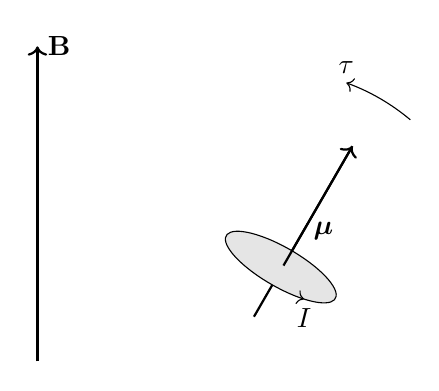
\begin{tikzpicture}
            \draw[->,thick] (240:0.5)--node[right]{\(\vb{\mu}\)}(60:2);
            \draw[->, rotate=-30, fill=gray!20] (0.38,0) arc [start angle=-60, end angle=305, x radius=0.8cm, y radius=0.25cm] node[below]{\(I\)};
            \draw[thick] (60:0.25)--(60:2);

            \draw[->,thick] (-3,-1)--(-3,3)node[right]{\(\vb{B}\)};
            \draw[->] (50:2.7) arc (50:70:2.7) node[above]{\(\tau\)};
        \end{tikzpicture}
        \caption{A charged particle with angular momentum will experience a torque in a magnetic field.}
    \end{figure}

    This reveals the close link between the angular momentum of a moving current and the magnetic moment. Suppose a particle of charge \(+q\) of mass \(m\) is rotating around a circle of radius \(r\) with angular velocity \(\vb{\omega}\). This is effectively a current
    \begin{equation}
        I=\frac{Q}{t}=\frac{\omega q}{2\pi}\,,
    \end{equation}
    which produces a magnetic moment
    \begin{equation}
        \vb{\mu} =\frac{\vb{\omega} q r^2}{2}\,.
    \end{equation}
    Since the particle carries an angular momentum
    \begin{equation}
        \vb{L}=mr^2\vb{\omega}\,,
    \end{equation}
    we can conclude that the magnetic moment it creates is proportional to the angular momentum
    \begin{equation}
        \vb{\mu}=\gamma\vb{L}=\frac{q}{2m}\vb{L}\,,
    \end{equation}
    where the proportionality constant \(\gamma\) is known as the \textit{gyromagnetic ratio}. This magnetic moment, coming from orbital angular momentum (momentum caused by particle orbiting around some point), is often written with a seemingly redundant extra factor
    \begin{equation}
        \vb{\mu}_{L}=g_L \frac{q}{2m}\vb{L}\,,
    \end{equation}
    where \(g_L=1\) is the Land\'{e} \(g\)-factor for orbital angular momentum for a reason that will be apparent immediately.

    Some charge-carrying particles, like electrons, have another natural source of angular momentum --- that is its spin. For a particle of spin \(S\), it carries a spin angular momentum of magnitude
    \begin{equation}
        \norm{\vb{S}}=\hbar\sqrt{S(S+1)}\,,
    \end{equation}
    which also leads to a magnetic moment
    \begin{equation}
        \vb{\mu}_S = \gamma \vb{S}=g_S \frac{q}{2m}\vb{S}\,.
    \end{equation}
    The spin of a particle does not come from its circular motion. It is intrinsic to the particle so we have no reason to assume \(g_S=1\) as for the orbital angular momentum case. For free electrons, \(g_{S, e-}\approx 2.0\),\footnote{In Dirac's theory, every point-like Fermion should have \(g_S=2\) exactly, while it is actually slightly above \(2\) for some subtle Quantum Field Theory effects. This is known as the anomalous magnetic moment.} while for other particles like a proton, it takes some other values that are not relevant for us. For a single, isolated free electron, the magnitude of the magnetic moment is
    \begin{equation}
        \mu_S=g_S\mu_{\text{B}}\sqrt{S(S+1)}\,,
    \end{equation}
    where \(S=\frac{1}{2}\), and \(\mu_{\text{B}}\) is the Bohr's magneton, characterising the strength of the magnetic moment of an electron. Note that since the charge of an electron is negative, \(q=-e\), its magnetic moment \(\vb{\mu}_S\) is in the opposite direction of its spin \(\vb{S}\), i.e. the gyromagnetic ratio is negative. We will take extra care on whether we are talking about the direction of the spin or the direction of the magnetic moment in future.

    \subsection{Magnetic Moment of Ions and Atoms}
    In an ion or atom, there are two main sources of angular momenta --- the spins and the orbital angular momentum of the electrons. The nucleus also carries nuclear spin, but the magnetic moment is proportional to \(m^{-1}\), and since nuclei are much heavier than the electrons, we are ignoring the nuclear contribution.

    The Schr\"{o}dinger equation tells us that the electronic spins and orbital angular momentum of an atom (ion) are characterised by two quantum numbers, the total spin quantum number \(S\) and the total orbital angular momentum quantum number \(L\). However, due to relativistic effects that are neglected in Schr\"{o}dinger's equation, the spin and orbital angular momentum can interact, and the effect is that these two numbers are no longer well defined. This process is called \textit{spin-orbit coupling}, and the overall result is that the spin is well-described by the total angular momentum quantum number \(J\).

    The strength of spin-orbit coupling is characterised by the spin-orbit coupling constant \(\lambda\), and the magnitude of \(\lambda\) is strongly dependent on the nuclear charge, \(\lambda\propto Z^4\). This means that for atoms not too heavy (up to around the third row transition metals), we can treat the spin-orbit coupling as a perturbation and still sensibly talk about the \(L\) and \(S\) values of an electronic term, and the possible \(J\) values are \(J=L+S, \dots, \abs{L-S}\). This is the \textit{\(LS\) coupling} (or \textit{Russell--Saunders coupling}) scheme. For the remainder of this course, we will always assume that the spin-orbit coupling is weak enough that the \(LS\) coupling scheme always applies.
    
    The way to work out the \(L\), \(S\) and \(J\) values for an electronic configuration should be familiar from Part IB and Part II, and the ground term (level) is determined by the Hund's rules.

    \begin{ex}
        \textit{Gaseous \(\mathrm{Ti^{3+}}\) ion.}

        A free \(\mathrm{Ti^{3+}}\) ion has electron configuration \(\mathrm{[Ar]\ 3d^1}\). The \(L\) and \(S\) values satisfying the Hund's first and second rules can be worked out using the box method.

        \begin{figure}[ht!]
            \centering
            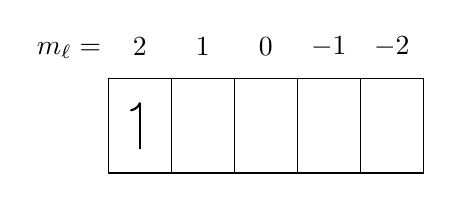
\begin{tikzpicture}
                \foreach \i in {-2,...,2}{
                    \draw (0.8*\i-0.4,-0.6) rectangle (0.8*\i + 0.4, 0.6);
                    \node at (-0.8*\i,1) {\(\i\)};
                }
                \draw[arrows = {->[left]}, thick] (-1.6,-0.3)--(-1.6,0.3);
                \node at (-2.5,0.95){\(m_\ell = \)};
            \end{tikzpicture}
        \end{figure}

        This gives \(L=2\) and \(S=\frac{1}{2}\), with spin multiplicity \(2S+1=2\). The available \(J\) values are \(J=\frac{5}{2}, \frac{3}{2}\). This is less than half-filled, so we need to minimise \(J\), giving \(J=\frac{3}{2}\). The ground level is therefore \(^2 D_{\frac{3}{2}}\).

        \begin{figure}[ht!]
            \centering
            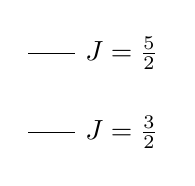
\begin{tikzpicture}
                \draw (-0.3,0)--(0.3,0)node[right]{\(J=\frac{3}{2}\)};
                \draw (-0.3,1)--(0.3,1)node[right]{\(J=\frac{5}{2}\)};
            \end{tikzpicture}
        \end{figure}
    \end{ex}
    
    \subsubsection{Free Ions}
    When both the electronic spin and angular momentum are present in a free ion (atom), the overall magnetic moment is proportional to the total angular momentum:
    \begin{equation}\label{free_ion_m_J}
        \mu_J = g_J\mu_{\text{B}}\sqrt{J(J+1)}\,,
    \end{equation}
    where the Land\'{e} \(g\)-factor for the total angular momentum is given by the complicated formula
    \begin{equation}
        g_{J}=g_{L}\frac{J(J+1)-S(S+1)+L(L+1)}{2J(J+1)}+g_{S}\frac{J(J+1)+S(S+1)-L(L+1)}{2J(J+1)}\,.
    \end{equation}
    We have \(g_L=1\), and if we take \(g_S=2\), the above equation simplifies to
    \begin{equation}\label{free_ion_g_J}
        g_{J}\approx 1 + \frac{J(J+1)+S(S+1)-L(L+1)}{2J(J+1)}\,.
    \end{equation}

    \subsubsection{Transition Metal Complexes}
    Free atoms and ions are of little interest to chemists. Instead, the materials showing the most interesting magnetic properties are the transition metal complexes, which will be the main topic of this course.

    The above equation cannot be directly applied to transition metal complexes, because we need a bit extra considerations on the orbital angular momentum.

    We now make the claim that for an ion to carry orbital angular momentum, it must have a set of partially filled degenerate orbitals. This can be seen from the atomic orbitals: an orbital with angular momentum quantum number \(\ell\) is \((2\ell+1)\)-degenerate, and the non-degenerate \(\mathrm{s}\)-orbital carries zero orbital angular momentum. The reason is that if several orbitals are degenerate, then any complex linear combination of them is also an allowed stationary state. The electron can occupy a coherent superposition with relative phases which evolve in a way such that it produces a probability density that circulates around the nucleus, leading to orbital angular momentum --- this can be imagined by electrons hopping between degenerate orbitals at different orientations.

    However, the degeneracies of the valence \(\mathrm{d}\) orbitals are broken in transition metal complexes due to ligand field splitting. This leads to the quenching of the orbital angular momentum. For example, in an octahedral complex, the \(\mathrm{d}\) orbitals are split into a \(T_{2g}\) set and a \(E_g\) set. The \(E_g\) set is only doubly degenerate, and since the orbital angular momentum quantum number can only be integers, it can carry no momentum. The \(T_{2g}\) set, on the other hand, are triply degenerate, and can carry one unit of angular momentum. Hence, if an octahedral complex has term symbol \(A\) or \(E\), it effectively has \(L_{\text{eff}}=0\), and we say that the angular momentum is completely quenched, while a complex with term symbol \(T\) is partially quenched, and has \(L_{\text{eff}}=1\).

    \begin{ex}
        \textit{Ground state term symbols and orbital angular momentum of octahedral complexes.}
        \begin{figure}[ht!]
            \centering
            \begin{tikzpicture}
                \draw (-1.6,0)--(-0.8,0);
                \draw (-0.4,0)--(0.4,0);
                \draw (0.8,0)--(1.6,0);
                \draw (-1,1.3)--(-0.2,1.3);
                \draw (0.2,1.3)--(1,1.3);
                \node at (-2.3,0) {\(t_{2g}\)};
                \node at (-2.3,1.3) {\(e_{g}\)};
                \foreach \i in {-1,0,1}{
                    \draw[arrows = {->[left]},thick] (1.2*\i-0.06,-0.2)--(1.2*\i-0.06,0.4);
                }
                \foreach \i in {-1,0}{
                    \draw[arrows = {->[left]},thick] (1.2*\i+0.06,0.4)--(1.2*\i+0.06,-0.2);
                }
                \foreach \i in {-1,0}{
                    \draw[arrows = {->[left]},thick] (1.2*\i+0.6-0.06,1.1)--(1.2*\i+0.6-0.06,1.7);
                }

                \node at (0,-1) {\(\mathrm{Co^{2+}}\), \(d^7\) HS};
                \node at (0,-1.55) {\(T\)};
                \node at (0,-2.1) {\(L_{\text{eff}}=1\).};

                \begin{scope}[shift={(5,0)}]
                    \draw (-1.6,0)--(-0.8,0);
                    \draw (-0.4,0)--(0.4,0);
                    \draw (0.8,0)--(1.6,0);
                    \draw (-1,1.3)--(-0.2,1.3);
                    \draw (0.2,1.3)--(1,1.3);
                    \foreach \i in {-1,0,1}{
                        \draw[arrows = {->[left]},thick] (1.2*\i-0.06,-0.2)--(1.2*\i-0.06,0.4);
                    }
                    \foreach \i in {-1}{
                        \draw[arrows = {->[left]},thick] (1.2*\i+0.6-0.06,1.1)--(1.2*\i+0.6-0.06,1.7);
                    }
                    \node at (0,-1) {\(\mathrm{Cr^{2+}}\), \(d^4\) HS};
                    \node at (0,-1.55) {\(E\)};
                    \node at (0,-2.1) {\(L_{\text{eff}}=0\).};
                \end{scope}

                \begin{scope}[shift={(10,0)}]
                    \draw (-1.6,0)--(-0.8,0);
                    \draw (-0.4,0)--(0.4,0);
                    \draw (0.8,0)--(1.6,0);
                    \draw (-1,1.3)--(-0.2,1.3);
                    \draw (0.2,1.3)--(1,1.3);
                    \foreach \i in {-1,0,1}{
                        \draw[arrows = {->[left]},thick] (1.2*\i-0.06,-0.2)--(1.2*\i-0.06,0.4);
                    }
                    \foreach \i in {-1,0}{
                        \draw[arrows = {->[left]},thick] (1.2*\i+0.6-0.06,1.1)--(1.2*\i+0.6-0.06,1.7);
                    }
                    \node at (0,-1) {\(\mathrm{Mn^{2+}}\), \(d^5\) HS};
                    \node at (0,-1.55) {\(A\)};
                    \node at (0,-2.1) {\(L_{\text{eff}}=0\).};
                \end{scope}
                
            \end{tikzpicture}
        \end{figure}
    \end{ex}

    To avoid this complication, it is often good enough to only consider the contribution of the electron spins to the magnetic moment. This leads to the spin only formula
    \begin{equation}
        \mu_{\text{so}}=g_{\text{so}}\mu_{\text{B}}\sqrt{S(S+1)}
    \end{equation}
    for an ion of spin quantum number \(S\). This is the formula you have seen throughout in Part IB and Part II when calculating the effective magnetic moment of e.g. a transition metal complex ion.

    If we are making a very crude estimation, then we can directly take the Land\'{e} \(g\)-factor to be that of a free electron, \(g_{\text{so}}\approx g_{S, e^-}\approx 2.0\). However, due to the fact that the electron is not completely free in the complexes and that we have ignored the orbital angular momentum contribution, we usually need a slightly larger value of \(g_{\text{so}}\) to match the experimental value of measured magnetic moment.
    \begin{ex}
        \textit{\(\mathrm{Ti^{3+}}\) complex: \(\mathrm{[Ti(CN)_6]^{3-}}\)}

        Let's return to the \(\mathrm{Ti^{3+}}\) example, but this time in a complex \(\mathrm{[Ti(CN)_6]^{3-}}\). Suppose this complex is octahedral, then the orbital diagram is shown below.

        \begin{figure}[ht!]
            \centering
            \begin{tikzpicture}
                \draw (-1.6,0)--(-0.8,0);
                \draw (-0.4,0)--(0.4,0);
                \draw (0.8,0)--(1.6,0);
                \draw (-1,1.7)--(-0.2,1.7);
                \draw (0.2,1.7)--(1,1.7);
                \node at (-2.3,0) {\(t_{2g}\)};
                \node at (-2.3,1.7) {\(e_{g}\)};
                \draw[arrows = {->[left]},thick] (-1.2,-0.2)--(-1.2,0.4);
                \node at (0,-1) {octahedral};

                \draw[dashed] (1,1.7)--(5,2);
                \draw[dashed] (1,1.7)--(5,1.3);
                \draw (5,2)--(5.8,2);
                \draw (5,1.3)--(5.8,1.3);
                \draw[dashed] (1,0)--(4.4,0.2);
                \draw[dashed] (1,0)--(5,-0.4);
                \draw (5,-0.4)--(5.8,-0.4);
                \draw (4.4,0.2)--(5.2,0.2);
                \draw (5.6,0.2)--(6.4,0.2);
                \draw[arrows = {->[left]},thick] (5.4,-0.6)--(5.4,0);
                \node at (5.4,-1) {distorted};
            \end{tikzpicture}
        \end{figure}

        The term symbol is \(^2 T_{2g}\), with \(L=1\) and \(S=\frac{1}{2}\). The available \(J\) values are \(\frac{1}{2}\) and \(\frac{3}{2}\).

        However, this complex has asymmetrically filled \(t_{2g}\) level, and so it is susceptible to Jahn--Teller distortion. This further breaks the degeneracy of the \(t_{2g}\) level and leads to a complete quenching of angular momentum.
    \end{ex}

    Due to the double effect of ligand field splitting and Jahn--Teller distortion, the orbital angular momentum of transition metal complexes are almost always completely quenched, and so it is fine to consider \(S\) only.

    \subsubsection{Lanthanide Ions}
    The special case comes to the lanthanide \(3^{+}\) ions. We have learned in Part II A1 that those ions have extremely contracted \(\mathrm{4f}\) orbitals, and the interactions between the metal ions and ligands are predominantly ionic with little covalency. As a result, the degeneracy of the \(\mathrm{4f}\) orbitals are not broken and they behave closely to free ions. Therefore, the formula of the magnetic moments and Land\'{e} \(g\)-factors for free ions, (\ref{free_ion_m_J}) and (\ref{free_ion_g_J}), work extremely well for lanthanide ions.

    \subsubsection{Spin Crossover Complex}
    We are familiar with the idea that a coordination complex can be classified as being either high or low spin. However, there are possibilities that the difference in crystal field stabilisation energies between the two spin states are so small that it is comparable to the thermal energy at some achievable temperature.
    
    The most common combination of metal and ligand that gives rise to this situation is \(\mathrm{Fe\ (II)}\) with moderately strong \(\sigma\)-donor ligands (e.g. \(\mathrm{S}\) or \(\mathrm{N}\)-donors). In these materials the low spin state (with \(S=0\)) is always lower in energy (enthalpy) than the high spin state (with \(S=2\)). However, a spin state \(S\) has degeneracy \(2S+1\), leading to an associated molar entropy
    \begin{equation}
        S_S=R\ln(2S+1)\,,
    \end{equation}
    where we have assumed the orbital angular momentum to be completely quenched. For free ions or lanthanide complexes where the orbital angular momentum is significant, the corresponding entropy is
    \begin{equation}
        S_J=R\ln(2J+1)\,.
    \end{equation}
    As the temperature is raised the population of the energetically excited state increases (from zero) and the sample switches from being diamagnetic to paramagnetic.

    For example, consider the octahedral \(\mathrm{Fe\ (II)}\) complex shown in \cref{Fig:crossover_structure} and the plot of \(\mu^2\) (or equivalently \(\chi T\), see later) against temperature is shown in \cref{Fig:crossover_plot}. The molecular orbital diagrams of the low spin and high spin states are shown below.

    \begin{figure}[ht!]
        \centering
        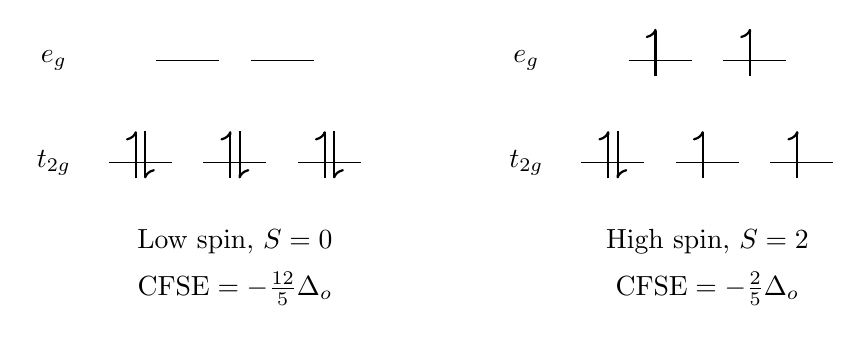
\begin{tikzpicture}
            \draw (-1.6,0)--(-0.8,0);
            \draw (-0.4,0)--(0.4,0);
            \draw (0.8,0)--(1.6,0);
            \draw (-1,1.3)--(-0.2,1.3);
            \draw (0.2,1.3)--(1,1.3);
            \node at (-2.3,0) {\(t_{2g}\)};
            \node at (-2.3,1.3) {\(e_{g}\)};
            \foreach \i in {-1,0,1}{
                \draw[arrows = {->[left]},thick] (1.2*\i-0.06,-0.2)--(1.2*\i-0.06,0.4);
            }
            \foreach \i in {-1,0,1}{
                \draw[arrows = {->[left]},thick] (1.2*\i+0.06,0.4)--(1.2*\i+0.06,-0.2);
            }

            \node at (0,-1) {Low spin, \(S=0\)};
            \node at (0,-1.6) {\(\mathrm{CFSE}=-\frac{12}{5}\Delta_o\)};

            \begin{scope}[shift={(6,0)}]
                \draw (-1.6,0)--(-0.8,0);
                \draw (-0.4,0)--(0.4,0);
                \draw (0.8,0)--(1.6,0);
                \draw (-1,1.3)--(-0.2,1.3);
                \draw (0.2,1.3)--(1,1.3);
                \node at (-2.3,0) {\(t_{2g}\)};
                \node at (-2.3,1.3) {\(e_{g}\)};
                \foreach \i in {-1,0,1}{
                    \draw[arrows = {->[left]},thick] (1.2*\i-0.06,-0.2)--(1.2*\i-0.06,0.4);
                }
                \foreach \i in {-1}{
                    \draw[arrows = {->[left]},thick] (1.2*\i+0.06,0.4)--(1.2*\i+0.06,-0.2);
                }
                \foreach \i in {-1,0}{
                    \draw[arrows = {->[left]},thick] (1.2*\i+0.6-0.06,1.1)--(1.2*\i+0.6-0.06,1.7);
                }

                \node at (0,-1) {High spin, \(S=2\)};
                \node at (0,-1.6) {\(\mathrm{CFSE}=-\frac{2}{5}\Delta_o\)};
            \end{scope}
        \end{tikzpicture}
    \end{figure}

    \begin{figure}[ht!]
        \centering
        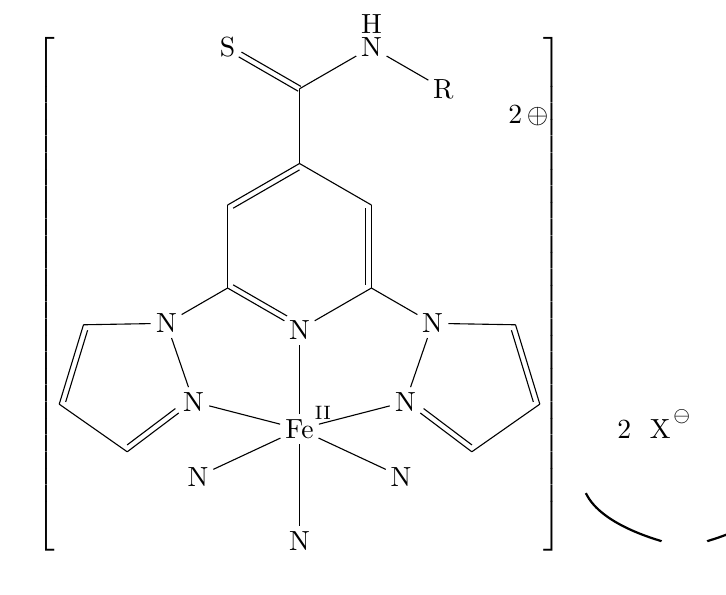
\begin{tikzpicture}
            \node at (0,0){
                \chemleft[\chemfig{
                    \charge{35:2.3pt=\scriptsize\(\mathrm{II}\)}{Fe}?[a]?[b]
                    (-[:90,1.2]  N*6(-[:60](-[,0.85]N*5([:-55]-N?[a]=-=-))=-(-[,0.9](=[:150]S)-[:30]\chemabove{N}{H}-[:-30]R)=-(-[,0.85]N*5([:-125]-=-=N?[b]-))=))
                    (-[:-90,1.35]@{c}N)
                    (-[:-155,1.35]@{d}N)
                    (-[:-25,1.35]@{e}N)
                }\chemright]\qquad 2 \ \chemfig{\charge{30:3pt=\scriptsize\(\ominus\)}{X}}
                \chemmove{\draw[-,thick,shorten <=1mm,shorten >=1mm](c)..controls +(180:2mm) and +(-65:7mm)..(d);}
                \chemmove{\draw[-,thick,shorten <=1mm,shorten >=1mm](c)..controls +(0:2mm) and +(-115:7mm)..(e);}
            };
            \node at (2.1,2.3) {\(2\,\oplus\)};
        \end{tikzpicture}
        \caption{The structure of a spin crossover complex, where \(\mathrm{R}\) is \(\mathrm{Me}\) or \(\mathrm{H}\) and \(\mathrm{X^-}\) is \(\mathrm{BF_4^-}\) or \(\mathrm{ClO_4^-}\).}
        \label{Fig:crossover_structure}
    \end{figure}

    \begin{figure}
        \centering
        % This file was created with matplot2tikz v0.4.0.
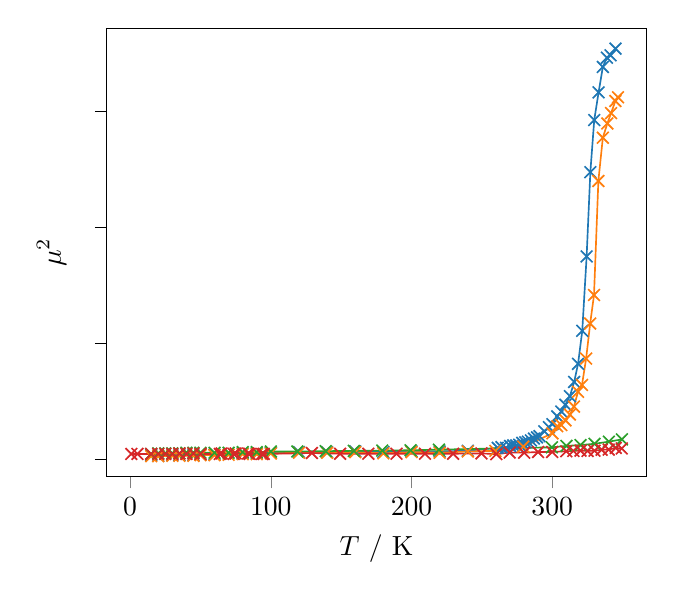
\begin{tikzpicture}

\definecolor{crimson2143940}{RGB}{214,39,40}
\definecolor{darkgray176}{RGB}{176,176,176}
\definecolor{darkorange25512714}{RGB}{255,127,14}
\definecolor{forestgreen4416044}{RGB}{44,160,44}
\definecolor{steelblue31119180}{RGB}{31,119,180}

\begin{axis}[
tick align=outside,
tick pos=left,
x grid style={darkgray176},
xlabel={\(\displaystyle T\) / \(\displaystyle \mathrm{K}\)},
xmin=-16.5854903156202, xmax=366.934851215292,
y grid style={darkgray176},
ylabel={\(\displaystyle \mu^2\)},
ymin=-3.04606060606061, ymax=74.2339393939394,
ytick style={color=black},
yticklabel=\empty,
]
\addplot [draw=steelblue31119180, fill=steelblue31119180, mark=x, only marks]
table{%
x  y
15 0.636363636363636
20 0.53030303030303
30 0.636363636363636
35 0.636363636363636
45 0.636363636363636
50 0.742424242424242
60 0.742424242424242
80 0.933333333333333
90 0.933333333333333
100 1.05
120 1.16666666666667
140 1.16666666666667
160 1.28333333333333
180 1.16666666666667
200 1.28333333333333
220 1.28333333333333
240 1.4
261.239711934156 1.90909090909091
263.940329218107 2.01515151515152
267.181069958848 1.90909090909091
270.061728395062 2.22727272727273
272.222222222222 2.33333333333333
274.382716049383 2.33333333333333
276.543209876543 2.43939393939394
278.703703703704 2.75757575757576
280.864197530864 2.86363636363636
282.664609053498 2.96969696969697
284.825102880658 3.18181818181818
286.985596707819 3.5
289.146090534979 3.71212121212121
290.946502057613 3.92424242424243
294.354569821328 4.76380344003295
297.6080247 5.46212121212121
300.128600823045 5.99242424242424
303.549382716049 7.31818181818182
306.430041152263 8.16666666666667
309.310699588477 9.33333333333333
312.551440329218 10.8181818181818
315.587306655314 13.2603187042842
318.343278463649 16.3831313131313
321.331447187929 22.0747474747475
324.434156378601 34.8939393939394
327.07475994513 49.4242424242424
329.839309367914 58.4075269085471
332.935913123656 63.1757982706972
335.956790123457 67.5606060606061
338.837448559671 69.1515151515152
341.442657877611 69.5590382257885
344.958847736626 70.7212121212121
};
\addplot [draw=darkorange25512714, fill=darkorange25512714, mark=x, only marks]
table{%
x  y
15 0.466666666666667
20 0.466666666666667
30 0.525
35 0.525
45 0.525
50 0.641666666666667
60 0.641666666666667
70 0.7
80 0.816666666666667
90 0.816666666666667
100 0.933333333333333
120 1.06060606060606
140 1.06060606060606
160 1.16666666666667
180 0.954545454545455
200 1.16666666666667
220 1.06060606060606
240 1.27272727272727
259.6193416 1.37878787878788
279.423868312757 2.12121212121212
300.128600823045 4.40151515151515
303.549382716049 5.62121212121212
306.430041152263 5.83333333333333
309.41081421494 6.64549161338152
312.551440329218 7.63636363636364
315.432098765432 9.01515151515151
318.312757201646 11.5606060606061
321.143935729133 12.7428829356366
324.074074074074 17.2878787878788
326.954732510288 23.3333333333333
329.682355967078 28.2479166666667
332.772232437323 47.9036643026005
335.956790123457 55.3636363636364
339.155082137241 57.8155333826066
341.806412894376 59.5979797979798
344.862090926906 61.6875901875902
346.73225308642 62.332702020202
};
\addplot [draw=forestgreen4416044, fill=forestgreen4416044, mark=x, only marks]
table{%
x  y
15 0.848484848484849
20 0.954545454545455
25 0.954545454545455
30 0.954545454545455
35 0.954545454545455
40 1.06060606060606
45 1.06060606060606
50 1.06060606060606
60 1.06060606060606
70 1.06060606060606
80 1.16666666666667
90 1.16666666666667
100 1.27272727272727
118.827160493827 1.27272727272727
138.991769547325 1.33113746157225
158.97633744856 1.37878787878788
179.16875773696 1.43483616654348
199.305555555556 1.48484848484848
219.470164609054 1.59090909090909
299.732510288066 1.98981481481482
310.081108240023 2.23467230443974
320.121170553269 2.38047138047138
330.055133481059 2.5998445998446
340.235907742368 2.96723044397463
349.502108418432 3.36120463898243
};
\addplot [draw=crimson2143940, fill=crimson2143940, mark=x, only marks]
table{%
x  y
0.847252481239409 0.848484848484849
5.22119341563786 0.848484848484849
15 0.848484848484849
20 0.848484848484849
25 0.848484848484849
30 0.848484848484849
35 0.932047750229577
40 0.848484848484849
45 0.932047750229577
50 0.848484848484849
63.7345679012346 0.848484848484849
65 0.932047750229577
73.649106808829 0.848484848484849
75 0.932047750229577
83.8991769547325 0.932047750229577
85 0.848484848484849
93.7789351851852 0.848484848484849
95 0.848484848484849
129.162379972565 1.00631313131313
149.258506473954 0.885802469135814
169.291636407649 0.885802469135814
189.316956657762 0.885802469135814
209.552725352002 0.885802469135814
229.552469135802 0.885802469135814
249.687738149672 0.940845959595966
260.262507441054 0.817800647989333
269.765275092138 1.08999634903249
280.033238366572 1.06831131831133
289.91224696486 1.18021334843766
299.948559670782 1.18916437098256
309.987891412217 1.31506422247163
315.001143118427 1.36902356902358
320.052509698069 1.42060388834583
325.117645938119 1.36798540965208
330.024744572158 1.41017938000697
335.078189300412 1.57676767676768
340.124229167439 1.60014560014561
345.124131417392 1.89605067064083
349.370967332216 1.79517396184063
};
\addplot [semithick, steelblue31119180, mark=x, mark size=3, mark options={solid}]
table {%
15 0.636363636363636
20 0.53030303030303
30 0.636363636363636
35 0.636363636363636
45 0.636363636363636
50 0.742424242424242
60 0.742424242424242
80 0.933333333333333
90 0.933333333333333
100 1.05
120 1.16666666666667
140 1.16666666666667
160 1.28333333333333
180 1.16666666666667
200 1.28333333333333
220 1.28333333333333
240 1.4
261.239711934156 1.90909090909091
263.940329218107 2.01515151515152
267.181069958848 1.90909090909091
270.061728395062 2.22727272727273
272.222222222222 2.33333333333333
274.382716049383 2.33333333333333
276.543209876543 2.43939393939394
278.703703703704 2.75757575757576
280.864197530864 2.86363636363636
282.664609053498 2.96969696969697
284.825102880658 3.18181818181818
286.985596707819 3.5
289.146090534979 3.71212121212121
290.946502057613 3.92424242424243
294.354569821328 4.76380344003295
297.6080247 5.46212121212121
300.128600823045 5.99242424242424
303.549382716049 7.31818181818182
306.430041152263 8.16666666666667
309.310699588477 9.33333333333333
312.551440329218 10.8181818181818
315.587306655314 13.2603187042842
318.343278463649 16.3831313131313
321.331447187929 22.0747474747475
324.434156378601 34.8939393939394
327.07475994513 49.4242424242424
329.839309367914 58.4075269085471
332.935913123656 63.1757982706972
335.956790123457 67.5606060606061
338.837448559671 69.1515151515152
341.442657877611 69.5590382257885
344.958847736626 70.7212121212121
};
\addplot [semithick, darkorange25512714, mark=x, mark size=3, mark options={solid}]
table {%
15 0.466666666666667
20 0.466666666666667
30 0.525
35 0.525
45 0.525
50 0.641666666666667
60 0.641666666666667
70 0.7
80 0.816666666666667
90 0.816666666666667
100 0.933333333333333
120 1.06060606060606
140 1.06060606060606
160 1.16666666666667
180 0.954545454545455
200 1.16666666666667
220 1.06060606060606
240 1.27272727272727
259.6193416 1.37878787878788
279.423868312757 2.12121212121212
300.128600823045 4.40151515151515
303.549382716049 5.62121212121212
306.430041152263 5.83333333333333
309.41081421494 6.64549161338152
312.551440329218 7.63636363636364
315.432098765432 9.01515151515151
318.312757201646 11.5606060606061
321.143935729133 12.7428829356366
324.074074074074 17.2878787878788
326.954732510288 23.3333333333333
329.682355967078 28.2479166666667
332.772232437323 47.9036643026005
335.956790123457 55.3636363636364
339.155082137241 57.8155333826066
341.806412894376 59.5979797979798
344.862090926906 61.6875901875902
346.73225308642 62.332702020202
};
\addplot [semithick, forestgreen4416044, mark=x, mark size=3, mark options={solid}]
table {%
15 0.848484848484849
20 0.954545454545455
25 0.954545454545455
30 0.954545454545455
35 0.954545454545455
40 1.06060606060606
45 1.06060606060606
50 1.06060606060606
60 1.06060606060606
70 1.06060606060606
80 1.16666666666667
90 1.16666666666667
100 1.27272727272727
118.827160493827 1.27272727272727
138.991769547325 1.33113746157225
158.97633744856 1.37878787878788
179.16875773696 1.43483616654348
199.305555555556 1.48484848484848
219.470164609054 1.59090909090909
299.732510288066 1.98981481481482
310.081108240023 2.23467230443974
320.121170553269 2.38047138047138
330.055133481059 2.5998445998446
340.235907742368 2.96723044397463
349.502108418432 3.36120463898243
};
\addplot [semithick, crimson2143940, mark=x, mark size=3, mark options={solid}]
table {%
0.847252481239409 0.848484848484849
5.22119341563786 0.848484848484849
15 0.848484848484849
20 0.848484848484849
25 0.848484848484849
30 0.848484848484849
35 0.932047750229577
40 0.848484848484849
45 0.932047750229577
50 0.848484848484849
63.7345679012346 0.848484848484849
65 0.932047750229577
73.649106808829 0.848484848484849
75 0.932047750229577
83.8991769547325 0.932047750229577
85 0.848484848484849
93.7789351851852 0.848484848484849
95 0.848484848484849
129.162379972565 1.00631313131313
149.258506473954 0.885802469135814
169.291636407649 0.885802469135814
189.316956657762 0.885802469135814
209.552725352002 0.885802469135814
229.552469135802 0.885802469135814
249.687738149672 0.940845959595966
260.262507441054 0.817800647989333
269.765275092138 1.08999634903249
280.033238366572 1.06831131831133
289.91224696486 1.18021334843766
299.948559670782 1.18916437098256
309.987891412217 1.31506422247163
315.001143118427 1.36902356902358
320.052509698069 1.42060388834583
325.117645938119 1.36798540965208
330.024744572158 1.41017938000697
335.078189300412 1.57676767676768
340.124229167439 1.60014560014561
345.124131417392 1.89605067064083
349.370967332216 1.79517396184063
};
\end{axis}

\end{tikzpicture}

        \caption{The \(\mu^2\) against \(T\) of a spin crossover complex. The blue and orange plots are for \(\mathrm{R=Me}\) and the green and red points are for \(\mathrm{R=H}\).}
        \label{Fig:crossover_plot}
    \end{figure}
    
    The low spin state in enthalpically favourable due to a higher \(\abs{\text{CFSE}}\). Assuming each pair of spin-parallel electrons contributes an exchange energy \(-K\), we can estimate the enthalpy change from low spin to high spin to be
    \begin{align}
        \Delta H_m&\approx\left[-\frac{2}{5}\Delta_o - \binom{5}{2}K\right]-\left[-\frac{12}{5}\Delta_o - 2\binom{3}{2}K\right]\notag\\
        &=2\Delta_o-4K>0\,,
    \end{align}
    where \(\Delta_o\) is the octahedral crystal field splitting energy. The high spin state is entropically favoured,
    \begin{equation}
        \Delta S_m\approx R\ln S_{\text{HS}}-R\ln S_{\text{LS}}=R\ln 5>0\,,
    \end{equation}
    which allows us to estimate the spin crossover temperature
    \begin{equation}
        \Delta G_m = \Delta_r H_m - T_c \Delta S_m =0 \quad\implies \quad T_c = \frac{\Delta H_m}{\Delta S_m}\,.
    \end{equation}

    Note that the identity of the \(\mathrm{R}\) group has an effect on the crossover temperature. This is because we have neglected the volumetric contribution to the enthalpy, \(\Delta H_m=\Delta E_m+P\Delta V_m\). There is an associated size change when the spin state of the complex changes. Due to the different sizes of the \(\mathrm{R}\) groups, the packing densities of the complexes in solid states might be different, and hence the \(\Delta V_m\) might be different. This leads to a change in \(\Delta H_m\) and hence in crossover temperature \(T_c\).

    \subsection{Magnetisation in Bulk Material}
    The magnetic moment of a single ion is, however, difficult to measure since practically we always have a bulk material, and what we can measure is only the combined magnetic properties of the whole sample. Here, we will assume that the magnetic moments of different spin carriers are non-interacting, so the total magnetic moment of the sample, known as the \textit{magnetisation}, is just the vector sum of all the individual magnetic moments of each ions,
    \begin{equation}
        \vb{M}=\sum\vb{\mu}\,.
    \end{equation}
    We will look at this in two different perspectives --- a classical perspective and a quantum perspective; the latter is apparently more correct.
    \subsubsection{The Classical View}
    Now suppose we have an ensemble of non-interacting magnetic moments that are allowed to point in any direction in space, as shown in \cref{Fig:Classical_magnetisation}. When there are no external magnetic fields, \(\vb{H}=\vb{0}\), the magnetic moments have no preferred orientations so they are pointing in random directions. Therefore, their vector sum cancels out by symmetry and we have \(\vb{M}=\vb{0}\) as shown in (a). Now suppose we are applying a small magnetic field in some direction, say \(\vu{z}\), \(\vb{H}=H\vu{z}\). The magnetic moments interact with the field with energy \(E=-\vb{H}\vdot\vb{\mu}\), so they are preferred to align with the field. However, temperature will randomize the orientations of the magnetic moments since the randomized state has larger entropy than having all spins completely aligned with the field. As a result, we have a small resultant magnetisation along the applied field, \(\vb{M}=M\vu{z}\), as shown in (b). As we increase the field, there are larger preference for the spins to align with the field since the energy penalty of misalignment increases, and so the \(M\) increases, as shown in (c). This comes to a limit when all the spins are completely aligned with the field as in (d), and we reach a saturation magnetisation \(\vb{M}_{\text{sat}}=M_{\text{sat}}\vu{z}\).

    \begin{figure}[ht!]
        \centering
        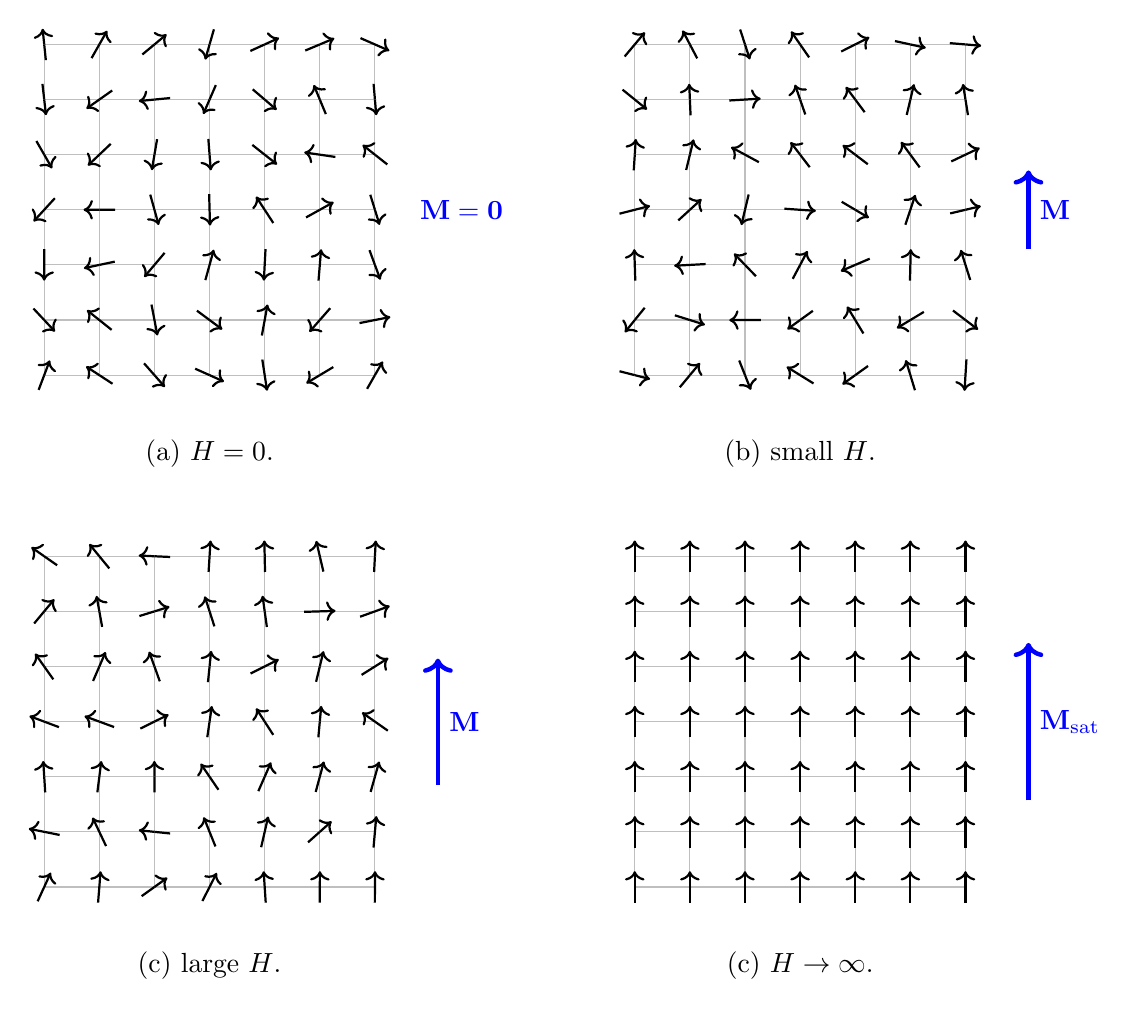
\begin{tikzpicture}
            \foreach \i in {0,...,6}{
                \draw[thin,color=gray!50] (0.7*\i,0)--(0.7*\i,4.2);
                \draw[thin,color=gray!50] (0,0.7*\i)--(4.2,0.7*\i);
            }
            \foreach \i in {0,...,6}{
                \foreach \j in {0,...,6}{
                    \tikzmath{\x = rand*180;}
                    \draw[thick] (0.7*\i,0.7*\j)--++(180+\x :0.2);
                    \draw[->,thick] (0.7*\i,0.7*\j)--++(\x :0.2);
                }
            }
            \node at (5.3,2.1)[blue]{\(\vb{M}=\vb{0}\)};
            \node at (2.1,-1){(a) \(H=0\).};
            \begin{scope}[shift={(7.5,0)}]
                \foreach \i in {0,...,6}{
                    \draw[thin,color=gray!50] (0.7*\i,0)--(0.7*\i,4.2);
                    \draw[thin,color=gray!50] (0,0.7*\i)--(4.2,0.7*\i);
                }
                \foreach \i in {0,...,6}{
                    \foreach \j in {0,...,6}{
                        \tikzmath{\x = rand;
                        \y = 70*\x + 110*\x*\x*\x + 90;}
                        \draw[thick] (0.7*\i,0.7*\j)--++(180+\y :0.2);
                        \draw[->,thick] (0.7*\i,0.7*\j)--++(\y :0.2);
                    }
                }
                \draw[ultra thick, blue, ->] (5,1.6)--node[right]{\(\vb{M}\)}(5,2.6);
                \node at (2.1,-1){(b) small \(H\).};
            \end{scope}
            \begin{scope}[shift={(0,-6.5)}]
                \foreach \i in {0,...,6}{
                    \draw[thin,color=gray!50] (0.7*\i,0)--(0.7*\i,4.2);
                    \draw[thin,color=gray!50] (0,0.7*\i)--(4.2,0.7*\i);
                }
                \foreach \i in {0,...,6}{
                    \foreach \j in {0,...,6}{
                        \tikzmath{\x = rand;
                        \y = 30*\x + 70*\x*\x*\x + 90;}
                        \draw[thick] (0.7*\i,0.7*\j)--++(180+\y :0.2);
                        \draw[->,thick] (0.7*\i,0.7*\j)--++(\y :0.2);
                    }
                }
                \draw[ultra thick, blue, ->] (5,1.3)--node[right]{\(\vb{M}\)}(5,2.9);
                \node at (2.1,-1){(c) large \(H\).};
            \end{scope}
            \begin{scope}[shift={(7.5,-6.5)}]
                \foreach \i in {0,...,6}{
                    \draw[thin,color=gray!50] (0.7*\i,0)--(0.7*\i,4.2);
                    \draw[thin,color=gray!50] (0,0.7*\i)--(4.2,0.7*\i);
                }
                \foreach \i in {0,...,6}{
                    \foreach \j in {0,...,6}{
                        \draw[thick] (0.7*\i,0.7*\j)--++(-90 :0.2);
                        \draw[->,thick] (0.7*\i,0.7*\j)--++(90 :0.2);
                    }
                }
                \draw[ultra thick, blue, ->] (5,1.1)--node[right]{\(\vb{M}_{\text{sat}}\)}(5,3.1);
                \node at (2.1,-1){(c) \(H\to\infty\).};
            \end{scope}
        \end{tikzpicture}
        \caption{Non-interacting magnetic moments at finite temperatures with magnetic fields upward.}
        \label{Fig:Classical_magnetisation}
    \end{figure}

    Since in a bulk material, each magnetic moment experiences an energy \(E=-\vb{\mu}\vdot\vb{H}=-\mu_z H\) in the magnetic field, and the magnetisation in other directions other that \(z\) cancels out so we have \(M=\sum \mu_z\), we can identify that\footnote{Technically, this should be Helmholtz (or Gibbs) free energy in \(NVT\) (\(NVP\)) ensembles.}
    \begin{equation}
        M=-\pdv{E}{H}\,.
    \end{equation}
    We further define the \textit{magnetic susceptibility}, \(\chi\), to be the ease that the magnetisation is generated by the magnetic field,
    \begin{equation}
        \chi\coloneqq \pdv{M}{H}=-\pdv[2]{E}{H}\,.
    \end{equation}
    By the crude analysis above, we can have the rough idea that the magnetic susceptibility is large near \(H=0\), while it decreases to \(0\) when \(H\) is very large, since then the magnetisation will reach a saturation and further increasing \(H\) will not increase \(M\) any more.
    
    \subsubsection{The Quantum View}
    Now let's proceed to the quantum mechanical view of magnetisation. Now when we impose a magnetic field of strength \(H\) along \(\vu{z}\) direction, what it does to a quantum mechanical spin is that it creates a preferred direction, or axis of quantisation. We can therefore observe the component of spins along this direction. For a particle of spin \(S\), its spin angular momentum along \(z\) direction spin governed by the spin magnetic quantum number, \(M_S\), taking values \(-S, -S+1, \dots, S\). There are in total \(2S+1\) of them. The spin angular momentum along this direction is \(S_z=\hbar M_S\). Since the field strength is \(H\), each of these levels have different energies
    \begin{equation}
        E=-\vb{\mu}\vdot\vb{H}=g\mu_{\text{B}} M_S H\,.
    \end{equation}
    The negative sign disappears because recall that the gyromagnetic ratio of electron is negative so the direction of spin is opposite to that of the magnetic moment. The magnetic field breaks the degeneracies of different \(M_S\) levels, and the energy gap between levels are proportional to \(H\).

    \begin{figure}
        \centering
        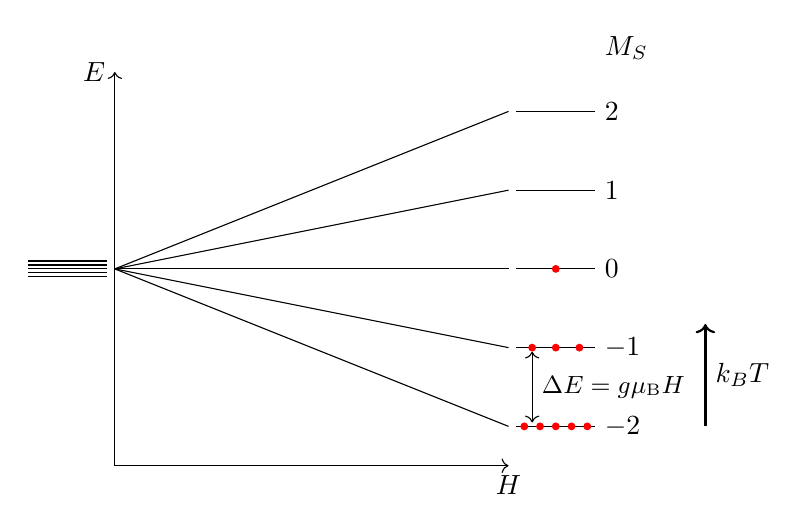
\begin{tikzpicture}
            \draw[->] (0,0)--(5,0)node[below]{\(H\)};
            \draw[->] (0,0)--(0,5)node[left]{\(E\)};
            \foreach \i in {-2,...,2}{
                \draw(0,2.5)--(5,2.5+\i);
                \draw (-1.1,2.5+0.05*\i)--(-0.1,2.5+0.05*\i);
                \draw (5.1,2.5+\i)--(6.1,2.5+\i)node[right]{\(\i\)};
            }
            \node at (6.1,5.3)[right]{\(M_S\)};
            \draw[<->](5.3,0.55)--node[right]{\small\(\Delta E=g\mu_{\text{B}}H\)}(5.3,1.45);
            \draw[thick,->] (7.5,0.5)--node[right]{\(k_B T\)}(7.5,1.8);
            \foreach \i in {-2,...,2}{
                \fill[red] (5.6+0.2*\i,0.5) circle (0.05);
            }
            \foreach \i in {-1,...,1}{
                \fill[red] (5.6+0.3*\i,1.5) circle (0.05);
            }
            \fill[red] (5.6,2.5) circle (0.05);
        \end{tikzpicture}
        \caption{External magnetic field results in the splitting of the \(M_S\) levels. The occupation of the \(M_S\) levels in the canonical ensemble follows the Boltzmann distribution.}
    \end{figure}

    The population of different \(M_S\) levels follows the Boltzmann distribution. When \(\Delta E=g\mu_{\text{B}} H\gg k_B T\), i.e. the magnetic field is large or the temperature is small, the spins will populate the lowest \(M_S\) state only. Therefore, the magnetic moments are maximally aligned with the field and we have a maximum \(\vb{M}=\vb{M}_{\text{sat}}\). If we decrease the field strength or increase the temperature, the thermal energy will be enough to promote the spins to higher \(M_S\) values, until when \(\Delta E=g\mu_{\text{B}} H\ll k_B T\), all \(M_S\) states are equally occupied, and the magnetic moments cancels so we get \(\vb{M}=\vb{0}\).

    \subsubsection{The Brillouin Function}
    We can be more quantitative. The canonical thermal average of the \(M_S\) value is
    \begin{align}
        \eval{M_S}&=\frac{\sum_{M_S=-S}^{S} M_S \ee^{-\beta E(M_S)}}{\sum_{M_S=-S}^{S} \ee^{-\beta E(M_S)}}\notag \\
        &=\frac{\sum_{M_S=-S}^{S} M_S \ee^{-\beta g\mu_{\text{B}} M_S H}}{\sum_{M_S=-S}^{S} \ee^{-\beta g\mu_{\text{B}} M_S H}}\,,
    \end{align}
    where \(\beta=1/k_B T\) is the thermodynamic inverse temperature. Denoting \(\beta g\mu_{\text{B}} H\) as \(\lambda\), this is
    \begin{align}
        \eval{M_S}&=\frac{\sum_{M_S=-S}^{S} M_S \ee^{-\lambda M_S}}{\sum_{M_S=-S}^{S} \ee^{-\lambda M_S}}\notag \\
        &=\frac{-\pdv{}{\lambda}\sum_{M_S=-S}^{S} \ee^{-\lambda M_S}}{\sum_{M_S=-S}^{S} \ee^{-\lambda M_S}}\notag \\
        &=-\pdv{}{\lambda}\ln Z(\lambda)\,,
    \end{align}
    where \(Z(\lambda)=\sum_{M_S}\ee^{-\lambda M_S}\) is the partition function. This partition function is a geometric series, evaluated to
    \begin{equation}
        Z(\lambda)=\frac{\sinh(\frac{(2S+1)\lambda}{2})}{\sinh(\frac{\lambda}{2})}\,,
    \end{equation}
    and finally this gives
    \begin{equation}
        \eval{M_S}=-\left[\frac{2S+1}{2}\coth\left(\frac{(2S+1)}{2}\lambda\right)-\frac{1}{2}\coth\left(\frac{\lambda}{2}\right)\right]\,.
    \end{equation}
    It's common to define the \textit{Brillouin function}
    \begin{equation}
        B_S(x)=\frac{2S+1}{2S}\coth\left(\frac{(2S+1)}{2S}x\right)-\frac{1}{2}\coth\left(\frac{x}{2S}\right)\,.
    \end{equation}
    This allows us to compactly write
    \begin{equation}
        \eval{M_S}=-SB_S(\lambda S)=-SB_S(\beta g\mu_{\text{B}}S H)\,.
    \end{equation}
    The molar magnetisation is therefore
    \begin{align}
        M(H, T) &= -N_A g \mu_{\text{B}}\eval{M_S}=N_A g \mu_{\text{B}} S B_S(\beta g\mu_{\text{B}}S H)\notag \\
        &=N_A g \mu_{\text{B}} S B_S\left(\frac{g\mu_{\text{B}}S}{k_B} \frac{H}{T}\right)\,.
    \end{align}
    where \(N_A\) is the Avogadro's constant.

    The magnetisation \(M\) is a function of \(\frac{H}{T}\) only, but the functional form in pretty complex. Their plots are shown in \cref{Fig:Brillouin_func}. These plots are, however, easy to interpret. As \(H/T\) increases, the molar magnetisation monotonically increases until it reaches the saturation value \(N_A g \mu_{\text{B}} S\), or \(2S\) molar Bohr magnetons taking \(g=2\). This gives us a way of measuring the spin in bulk magnetic materials.

    \begin{figure}
        \centering
        % This file was created with matplot2tikz v0.4.0.
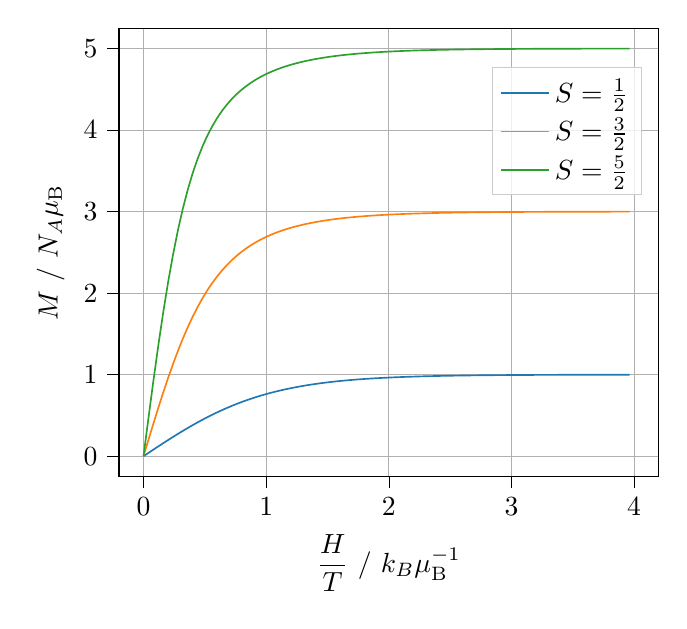
\begin{tikzpicture}

\definecolor{darkgray176}{RGB}{176,176,176}
\definecolor{darkorange25512714}{RGB}{255,127,14}
\definecolor{forestgreen4416044}{RGB}{44,160,44}
\definecolor{lightgray204}{RGB}{204,204,204}
\definecolor{steelblue31119180}{RGB}{31,119,180}

\begin{axis}[
legend cell align={left},
legend style={
  fill opacity=0.8,
  draw opacity=1,
  text opacity=1,
  at={(0.97,0.77)},
  anchor=east,
  draw=lightgray204
},
tick align=outside,
tick pos=left,
x grid style={darkgray176},
xlabel={\(\displaystyle \frac{H}{T}\) / \(\displaystyle k_B \mu_{\text{B}}^{-1}\) },
xmajorgrids,
xmin=-0.1999895, xmax=4.1999995,
xtick style={color=black},
y grid style={darkgray176},
ylabel={\(\displaystyle M\) / \(\displaystyle N_A\mu_{\text{B}}\) },
ymajorgrids,
ymin=-0.249953433730955, ymax=5.24924210842453,
ytick style={color=black}
]
\addplot [semithick, steelblue31119180]
table {%
1e-05 1.00000033853576e-05
0.0400499399399399 0.0400285403327665
0.0800898798798799 0.0799190755642059
0.12012981981982 0.11955526476503
0.16016975975976 0.158813986856416
0.2002096996997 0.19757684230597
0.24024963963964 0.235731530734823
0.28028957957958 0.273173071885133
0.32032951951952 0.309804844167731
0.360369459459459 0.345539422587116
0.400409399399399 0.380299205760097
0.440449339339339 0.414016829551124
0.480489279279279 0.446635372133679
0.520529219219219 0.478108361717756
0.560569159159159 0.508399603513739
0.600609099099099 0.537482846585722
0.640649039039039 0.565341314030664
0.680688978978979 0.591967121437393
0.720728918918919 0.61736060893463
0.760768858858859 0.641529611484504
0.800808798798799 0.664488690603608
0.840848738738739 0.686258348597395
0.880888678678679 0.706864243873452
0.920928618618619 0.72633642313831
0.960968558558558 0.744708583441805
1.0010084984985 0.762017374245393
1.04104843843844 0.778301747059531
1.08108837837838 0.793602357794332
1.12112831831832 0.807961024844575
1.16116825825826 0.821420244109127
1.2012081981982 0.834022760631165
1.24124813813814 0.845811195329749
1.28128807807808 0.856827724355468
1.32132801801802 0.867113807915651
1.36136795795796 0.876709964947284
1.4014078978979 0.88565558973565
1.44144783783784 0.89398880645176
1.48148777777778 0.901746357581712
1.52152771771772 0.908963522318369
1.56156765765766 0.915674061155857
1.6016075975976 0.921910183149198
1.64164753753754 0.927702532557095
1.68168747747748 0.933080191860988
1.72172741741742 0.938070698436296
1.76176735735736 0.94270007243322
1.8018072972973 0.946992853697771
1.84184723723724 0.950972145823939
1.88188717717718 0.954659665671765
1.92192711711712 0.958075796911516
1.96196705705706 0.961239646360128
2.002006996997 0.96416910206231
2.04204693693694 0.966880892235553
2.08208687687688 0.969390644346519
2.12212681681682 0.971712943716875
2.16216675675676 0.973861391170903
2.2022066966967 0.975848659336443
2.24224663663664 0.977686547296259
2.28228657657658 0.979386033360161
2.32232651651652 0.980957325790467
2.36236645645646 0.982409911365875
2.4024063963964 0.98375260171272
2.44244633633634 0.984993577369004
2.48248627627628 0.986140429576454
2.52252621621622 0.987200199820076
2.56256615615616 0.988179417154061
2.6026060960961 0.989084133368128
2.64264603603604 0.989919956060087
2.68268597597598 0.990692079689135
2.72272591591592 0.991405314690667
2.76276585585586 0.992064114737498
2.8028057957958 0.992672602234891
2.84284573573574 0.993234592137772
2.88288567567568 0.993753614178452
2.92292561561562 0.994232933592137
2.96296555555556 0.994675570425765
3.0030054954955 0.995084317513429
3.04304543543544 0.995461757198906
3.08308537537538 0.995810276882782
3.12312531531532 0.99613208346844
3.16316525525526 0.99642921677777
3.2032051951952 0.996703562004026
3.24324513513514 0.996956861265775
3.28328507507507 0.997190724322442
3.32332501501502 0.997406638508551
3.36336495495495 0.997605977940441
3.40340489489489 0.997790012046037
3.44344483483483 0.997959913465137
3.48348477477477 0.998116765364713
3.52352471471471 0.998261568210856
3.56356465465465 0.99839524603632
3.60360459459459 0.998518652239996
3.64364453453453 0.998632574952266
3.68368447447447 0.998737741997828
3.72372441441441 0.998834825485462
3.76376435435435 0.998924446052126
3.80380429429429 0.999007176786888
3.84384423423423 0.999083546858359
3.88388417417417 0.99915404486767
3.92392411411411 0.999219121947386
3.96396405405405 0.999279194625354
};
\addlegendentry{\(S=\frac{1}{2}\)}
\addplot [semithick, darkorange25512714]
table {%
1e-05 5.00000169267878e-05
0.0400499399399399 0.199886563704123
0.0800898798798799 0.397566544808427
0.12012981981982 0.591037214803055
0.16016975975976 0.77844175555503
0.2002096996997 0.958192361211386
0.24024963963964 1.12901828526756
0.28028957957958 1.28998710943408
0.32032951951952 1.4405010799361
0.360369459459459 1.58027301769753
0.400409399399399 1.7092877559887
0.440449339339339 1.82775532408611
0.480489279279279 1.93606144713346
0.520529219219219 2.03471974070326
0.560569159159159 2.12432859712643
0.600609099099099 2.20553445591797
0.640649039039039 2.27900207962106
0.680688978978979 2.34539167888414
0.720728918918919 2.40534223748253
0.760768858858859 2.45946013179595
0.800808798798799 2.50831205850662
0.840848738738739 2.55242131952234
0.880888678678679 2.59226661505037
0.920928618618619 2.62828262780755
0.960968558558558 2.66086181906445
1.0010084984985 2.69035698591529
1.04104843843844 2.71708424137645
1.08108837837838 2.74132617200591
1.12112831831832 2.76333500200877
1.16116825825826 2.78333565013716
1.2012081981982 2.80152860866664
1.24124813813814 2.81809260501829
1.28128807807808 2.83318702868773
1.32132801801802 2.84695412120146
1.36136795795796 2.85952093663526
1.4014078978979 2.87100108622463
1.44144783783784 2.88149628388128
1.48148777777778 2.89109771084132
1.52152771771772 2.89988721783218
1.56156765765766 2.90793838250864
1.6016075975976 2.91531743879613
1.64164753753754 2.92208409341405
1.68168747747748 2.92829224338717
1.72172741741742 2.93399060688598
1.76176735735736 2.93922327833107
1.8018072972973 2.94403021738719
1.84184723723724 2.94844768027755
1.88188717717718 2.95250860077461
1.92192711711712 2.9562429272692
1.96196705705706 2.95967792147751
2.002006996997 2.96283842360938
2.04204693693694 2.96574708817852
2.08208687687688 2.96842459407879
2.12212681681682 2.97088983206766
2.16216675675676 2.97316007238181
2.2022066966967 2.97525111485019
2.24224663663664 2.97717742356014
2.28228657657658 2.97895224786527
2.32232651651652 2.98058773129364
2.36236645645646 2.98209500971685
2.4024063963964 2.9834842999692
2.44244633633634 2.98476497995871
2.48248627627628 2.98594566118419
2.52252621621622 2.98703425446182
2.56256615615616 2.98803802956936
2.6026060960961 2.98896366943256
2.64264603603604 2.9898173194066
2.68268597597598 2.99060463214193
2.72272591591592 2.99133080846941
2.76276585585586 2.99200063469117
2.8028057957958 2.99261851662203
2.84284573573574 2.99318851068902
2.88288567567568 2.99371435236413
2.92292561561562 2.99419948217693
2.96296555555556 2.99464706952845
3.0030054954955 2.99506003450495
3.04304543543544 2.99544106787105
3.08308537537538 2.99579264940344
3.12312531531532 2.99611706471119
3.16316525525526 2.99641642067442
3.2032051951952 2.99669265962077
3.24324513513514 2.99694757234796
3.28328507507507 2.99718281009058
3.32332501501502 2.9973998955204
3.36336495495495 2.99760023286144
3.40340489489489 2.99778511719367
3.44344483483483 2.99795574301266
3.48348477477477 2.9981132121067
3.52352471471471 2.99825854080741
3.56356465465465 2.9983926666651
3.60360459459459 2.99851645459575
3.64364453453453 2.99863070254237
3.68368447447447 2.99873614669015
3.72372441441441 2.99883346627101
3.76376435435435 2.99892328799094
3.80380429429429 2.99900619010985
3.84384423423423 2.99908270620193
3.88388417417417 2.99915332862193
3.92392411411411 2.99921851170051
3.96396405405405 2.99927867469033
};
\addlegendentry{\(S=\frac{3}{2}\)}
\addplot [semithick, forestgreen4416044]
table {%
1e-05 0.000116666651592823
0.0400499399399399 0.465410730451694
0.0800898798798799 0.919916025167318
0.12012981981982 1.35397336040696
0.16016975975976 1.75992727432049
0.2002096996997 2.13259508828216
0.24024963963964 2.46930417880385
0.28028957957958 2.76958798015103
0.32032951951952 3.03468720683061
0.360369459459459 3.26699893362712
0.400409399399399 3.46957590986467
0.440449339339339 3.64572922460578
0.480489279279279 3.79874727015762
0.520529219219219 3.93171922546803
0.560569159159159 4.04744047402031
0.600609099099099 4.14837588988802
0.640649039039039 4.23666025806247
0.680688978978979 4.31412006041967
0.720728918918919 4.38230568310684
0.760768858858859 4.44252703369128
0.800808798798799 4.49588844062335
0.840848738738739 4.54332066507465
0.880888678678679 4.58560909769225
0.920928618618619 4.62341794901883
0.960968558558558 4.65731064244815
1.0010084984985 4.68776680776602
1.04104843843844 4.71519633748108
1.08108837837838 4.73995096319464
1.12112831831832 4.76233376991595
1.16116825825826 4.78260701303354
1.2012081981982 4.80099854706472
1.24124813813814 4.81770712319869
1.28128807807808 4.83290676660705
1.32132801801802 4.84675040525176
1.36136795795796 4.8593728892441
1.4014078978979 4.87089351301895
1.44144783783784 4.88141813085275
1.48148777777778 4.89104093873653
1.52152771771772 4.89984598155591
1.56156765765766 4.90790843327096
1.6016075975976 4.91529568877739
1.64164753753754 4.92206829891568
1.68168747747748 4.92828077431004
1.72172741741742 4.93398227907167
1.76176735735736 4.939217231658
1.8018072972973 4.94402582715621
1.84184723723724 4.94844449280952
1.88188717717718 4.95250628661278
1.92192711711712 4.95624124717897
1.96196705705706 4.95967670174724
2.002006996997 4.96283753810959
2.04204693693694 4.96574644533163
2.08208687687688 4.9684241273959
2.12212681681682 4.97088949327642
2.16216675675676 4.97315982643623
2.2022066966967 4.97525093630715
2.24224663663664 4.97717729394841
2.28228657657658 4.97895215377524
2.32232651651652 4.98058766299044
2.36236645645646 4.98209496013338
2.4024063963964 4.98348426397508
2.44244633633634 4.98476495382957
2.48248627627628 4.98594564221636
2.52252621621622 4.98703424069261
2.56256615615616 4.98803801957396
2.6026060960961 4.98896366217667
2.64264603603604 4.98981731413939
2.68268597597598 4.99060462831835
2.72272591591592 4.99133080569379
2.76276585585586 4.99200063267629
2.8028057957958 4.9926185151594
2.84284573573574 4.99318850962727
2.88288567567568 4.99371435159338
2.92292561561562 4.99419948161743
2.96296555555556 4.9946470691223
3.0030054954955 4.99506003421011
3.04304543543544 4.99544106765702
3.08308537537538 4.99579264924808
3.12312531531532 4.99611706459841
3.16316525525526 4.99641642059255
3.2032051951952 4.99669265956134
3.24324513513514 4.99694757230482
3.28328507507507 4.99718281005926
3.32332501501502 4.99739989549766
3.36336495495495 4.99760023284493
3.40340489489489 4.99778511718169
3.44344483483483 4.99795574300397
3.48348477477477 4.99811321210039
3.52352471471471 4.99825854080283
3.56356465465465 4.99839266666177
3.60360459459459 4.99851645459333
3.64364453453453 4.99863070254062
3.68368447447447 4.99873614668887
3.72372441441441 4.99883346627009
3.76376435435435 4.99892328799027
3.80380429429429 4.99900619010936
3.84384423423423 4.99908270620158
3.88388417417417 4.99915332862167
3.92392411411411 4.99921851170032
3.96396405405405 4.99927867469019
};
\addlegendentry{\(S=\frac{5}{2}\)}
\end{axis}

\end{tikzpicture}

        \caption{The magnetisation per mole of non-interacting spins against \(H/T\), taking \(g=2\).}
        \label{Fig:Brillouin_func}
    \end{figure}

    This high \(H/T\) limit is, however, difficult to reach since we either need a really strong magnet or a temperature close to absolute zero --- both are experimentally inaccessible. We will go to this regime in experiments only if we really need to. Instead, we are more interested in the \(H/T\to 0\) limit, since a small magnetic field and room temperature are trivially achievable.

    \subsubsection{The Curie's Law}
    If you look carefully, you can see that the \(M(\frac{H}{T})\) graph is approximately linear in the \(\frac{H}{T}\to 0\) limit, which means a constant magnetic susceptibility. The full expression of \(\chi(H, T)=\pdv{M}{H}\) needs a tough differentiation of the Brillouin function, and its full expression is meaningless to us. Instead, to look at the \(\frac{H}{T}\to 0\) limit, we only need to perform a Taylor expansion in \(\frac{H}{T}\). For small \(x\), we have \(\coth x\sim\frac{1}{x}+\frac{1}{3}x\), and substituting into the expression of \(M\), we have
    \begin{equation}
        M(H, T)=\frac{N_A g^2 \mu_{\text{B}}^2 H S(S+1)}{3k_B T}\,.
    \end{equation}
    This means that for small \(H/T\), the magnetic susceptibility is
    \begin{equation}
        \chi=\frac{M}{H}=\frac{N_A g^2 \mu_{\text{B}}^2 S(S+1)}{3k_B T}\,.
    \end{equation}
    This is independent of \(H\) (as long as \(H\) is small) and inversely proportional to \(T\). We can write this as
    \begin{equation}
        \chi=\frac{C}{T}\,,
    \end{equation}
    which is known as \textit{Curie's law}, named after Pierre Curie (not Marie Curie), where
    \begin{equation}
        C=\frac{N_A g^2 \mu_{\text{B}}^2 S(S+1)}{3 k_B}
    \end{equation}
    is \textit{Curie's constant}. This law holds when
    \begin{itemize}
        \item the ground term is well isolated from any excited terms, so only the \(2S+1\) different \(M_S\) states from the same \(S\) state are populated at the temperature considered;
        \item there are no interactions between spins.
    \end{itemize}

    Note that we have \(\chi T=C\propto S(S+1)\), and we also have \(\mu^2\propto S(S+1)\), so it is actually the macroscopic quantity \(\chi T\) that is actually measured in experiments, not the microscopic \(\mu^2\). Therefore, in figures like \cref{Fig:crossover_plot}, the proper \(y\)-axis label should actually be \(\chi T\), not \(\mu^2\).

    \subsubsection*{A Note on Units}
    Whilst much of the scientific world has moved to SI units, magnetochemists have continued to work with the cgs (centimetre-gram-second) units. There is good reason to do this since it simplifies the calculations considerably.

    Before we proceed, let's make clear of two easily confused quantities, the magnetic flux density (or magnetic induction) \(\vb{B}\) and the magnetic field strength \(\vb{H}\). What we've discussed above is the magnetic field strength \(\vb{H}\), which measures the external magnetic field generated by free currents, not counting materials' response. However, when a external field is applied to a medium, the media respond to the external field and generates a magnetisation \(\vb{M}\). This magnetisation also generates magnetic fields that can be experienced by other particles in the media, such as a moving charge or other magnetic moments. The total effect is the magnetic flux density
    \begin{equation}
        \vb{B}=\mu_0(\vb{H}+\vb{M})\,,
    \end{equation}
    where in SI units, the vacuum magnetic permeability \(\mu_0=4\pi\times 10^{-7}\unit{N}\unit{A}^{-2}\). The SI unit of \(\vb{B}\) is Tesla (\(\mathrm{T}=\mathrm{kg\ s^{-2}\ A^{-2}}\)) and the unit of \(\vb{H}\) is \(\mathrm{A\ m^{-1}}\). Therefore in vacuum, we have an annoying scaling between \(\vb{B}\) and \(\vb{H}\):
    \begin{equation}
        \vb{B}=\mu_0\vb{H}\,.
    \end{equation}

    In the cgs unit, however, we take a different convention to move this extra \(4\pi\) factor in front of \(\vb{H}\) to somewhere in the Maxwell's equations (which doesn't affect us since we don't bother solving Maxwell's equations) so that now we have
    \begin{equation}
        \vb{B}_{\text{cgs}}=\vb{H}_{\text{cgs}}+4\pi\vb{M}_{\text{cgs}}\,,
    \end{equation}
    and in vacuum, we have
    \begin{equation}
        \vb{B}_{\text{cgs}}=\vb{H}_{\text{cgs}}
    \end{equation}
    so the magnetic field and magnetic flux density now becomes the same. The cgs unit of \(\vb{B}\) is Gauss (\(\mathrm{G}\)), with \(1\unit{T}=10,000\unit{G}\), and the unit of \(\vb{H}\) is Oersted (\(\mathrm{Oe}\)), so a magnetic field of \(1\unit{Oe}\) produces a magnetic flux density \(1\unit{G}\) in vacuum. The down side is that people often forget which is the correct unit of which, and tend to use them interchangeably.

    Two additional units in the cgs system are the energy \(1\unit{erg}=10^{-7}\unit{J}\) and the \textit{electromagnetic unit} for magnetic moments \(1\unit{emu}\equiv 1\unit{erg}\unit{G}^{-1}=10^{-3}\unit{J}\unit{T}^{-1}\). One mole of Bohr magnetons is \(N_A\mu_{\text{B}}=5,585\unit{emu}\unit{mol}^{-1}\) in cgs units, and the saturation magnetisation is
    \begin{equation}
        M_{\text{sat}}=g S N_A\mu_{\text{B}}\approx 5,585gS\unit{emu}\unit{mol}^{-1}\,.
    \end{equation}
    The combination of constants \(N_A \mu_{\text{B}}^2/3k_B=0.12504\unit{emu}\unit{K}\unit{mol}^{-1}\) is coincidentally very close to \(\frac{1}{8}\) in cgs units, which allows us to approximate the Curie's constant as
    \begin{equation}
        C=\frac{N_A \mu_{\text{B}}^2}{3k_B}g^2 S(S+1)\approx \frac{1}{8}g^2 S(S+1)\unit{emu}\unit{K}\unit{mol}^{-1}
    \end{equation}
    in cgs units. If we take \(g\approx 2\), this gives us the handy formula
    \begin{equation}
        C\approx\frac{1}{2}S(S+1)\unit{emu}\unit{K}\unit{mol}^{-1}\,.
    \end{equation}

    \subsubsection{Deviation from Curie Behaviour}
    In many compounds, the magnetic susceptibility does not obey the Curie law, but instead obey a modified version
    \begin{equation}
        \chi=\frac{C}{T-\Theta}
    \end{equation}
    known as the \textit{Curie--Weiss} law for some parameter \(\Theta\) known as the \textit{Weiss constant}. This deviation from the pure Curie law can arise from a series of phenomena, including the presence of thermally accessible excited states of a single ion or some form of interaction between spin centres on neighbouring molecules. We will look at mechanisms through which they can interact later, and we will have a glimpse of how this equation arise when we introduce the Ising model. What is important is that, in both situations, there is no longer a single energy level, so our above derivation for Curie law fails.

    Suppose we have two spins, quantised along some direction in the magnetic field. There are two possibilities of their relative alignments: they are either be parallel or antiparallel. If the spins are parallel, then they are said to be in \textit{ferromagnetic alignment}, and if they are antiparallel, they are in \textit{antiferromagnetic alignment}.

    If the interaction between the two spins have an effect such that the ferromagnetic (parallel) alignment is lowered in energy than having two isolated spins and the antiferromagnetic (antiparallel) spin is raised in energy, then the two spins are said to have a \textit{ferromagnetic interaction}. This types of interaction will encourage the alignment of spins with each other, and hence all of them tends to align with the field, leading to an increased magnetic susceptibility. This will lead to a positive \(\Theta\).

    On the other hand, if the interaction between spins has an effect to encourage antiferromagnetic alignment, then this is known as an antiferromagnetic interaction, which leads to a negative \(\Theta\).

    A plot of \(\chi\), \(\chi^{-1}\) and \(\chi T\) against \(T\) are shown in \cref{Fig:Curie_Weiss}. In the \(\chi^{-1}\)-\(T\) graph, it is easy to read off the value of \(\Theta\) by the \(x\) intercept, while in the \(\chi T\)-\(T\) graph, we have \(\chi T\to T\) as \(T\to\infty\) independent of \(\Theta\), which helps us to determine the spin \(S\) (or \(g\) value) of the molecule of interest.

    \begin{figure}
        \centering
        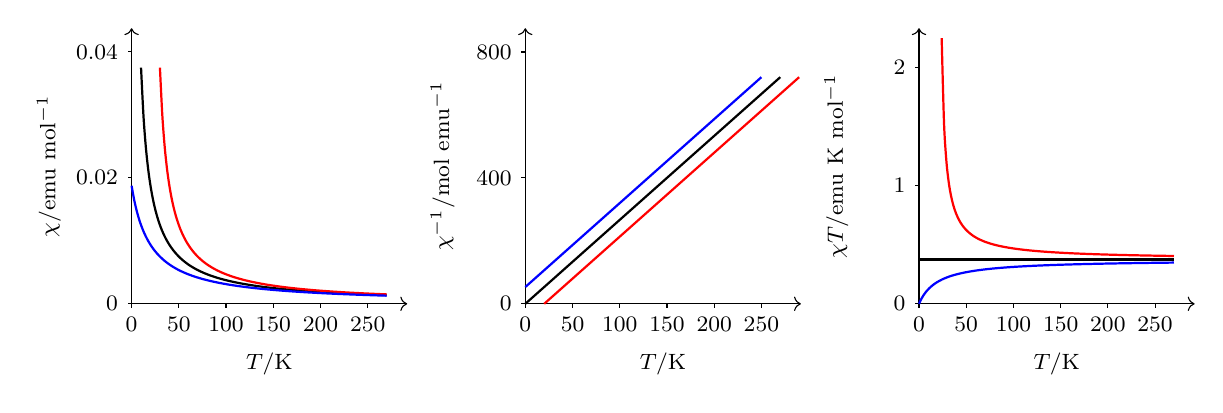
\begin{tikzpicture}
            \draw[->] (0,0)--node[below=5mm]{\footnotesize\(T/\mathrm{K}\)}(3.5,0);
            \draw[->] (0,0)--(0,3.5);
            \node[rotate=90] at (-1.05,1.75){\footnotesize\(\chi/\mathrm{emu\ mol^{-1}}\)};
            \foreach \i in {0,50,...,250}{
                \draw (0.012*\i, 0)--(0.012*\i, -0.05)node[below]{\footnotesize\(\i\)};
            }
            \foreach \i in {0,0.02,0.04}{
                \draw (0,80*\i)--(-0.05,80*\i)node[left]{\footnotesize\(\i\)};
            }
            \draw[thick,domain=10:270, smooth, variable=\x,samples=100] plot ({0.012*\x}, {80*0.375/\x});
            \draw[thick,domain=30:270, smooth, variable=\x,samples=100,red] plot ({0.012*\x}, {80*0.375/(\x-20)});
            \draw[thick,domain=0:270, smooth, variable=\x,samples=100,blue] plot ({0.012*\x}, {80*0.375/(\x+20)});

            \begin{scope}[shift={(5,0)}]
                \draw[->] (0,0)--node[below=5mm]{\footnotesize\(T/\mathrm{K}\)}(3.5,0);
                \draw[->] (0,0)--(0,3.5);
                \node[rotate=90] at (-1.05,1.75){\footnotesize\(\chi^{-1}/\mathrm{mol\ emu^{-1}}\)};
                \foreach \i in {0,50,...,250}{
                    \draw (0.012*\i, 0)--(0.012*\i, -0.05)node[below]{\footnotesize\(\i\)};
                }
                \foreach \i in {0,400,800}{
                    \draw (0,0.004*\i)--(-0.05,0.004*\i)node[left]{\footnotesize\(\i\)};
                }
                \draw[thick,domain=0:270, smooth, variable=\x,samples=100] plot ({0.012*\x}, {0.004*\x/0.375});
                \draw[thick,domain=20:290, smooth, variable=\x,samples=100,red] plot ({0.012*\x}, {0.004*(\x-20)/0.375});
                \draw[thick,domain=0:250, smooth, variable=\x,samples=100,blue] plot ({0.012*\x}, {0.004*(\x+20)/0.375});
            \end{scope}
            \begin{scope}[shift={(10,0)}]
                \draw[->] (0,0)--node[below=5mm]{\footnotesize\(T/\mathrm{K}\)}(3.5,0);
                \draw[->] (0,0)--(0,3.5);
                \node[rotate=90] at (-1.05,1.75){\footnotesize\(\chi T/\mathrm{emu\ K\ mol^{-1}}\)};
                \foreach \i in {0,50,...,250}{
                    \draw (0.012*\i, 0)--(0.012*\i, -0.05)node[below]{\footnotesize\(\i\)};
                }
                \foreach \i in {0,1,2}{
                    \draw (0,1.5*\i)--(-0.05,1.5*\i)node[left]{\footnotesize\(\i\)};
                }
                \draw[thick,domain=0:270, smooth, variable=\x,samples=100] plot ({0.012*\x}, {1.5*0.375});
                \draw[thick,domain=24:270, smooth, variable=\x,samples=100,red] plot ({0.012*\x}, {1.5*0.375*\x/(\x-20)});
                \draw[thick,domain=0:270, smooth, variable=\x,samples=100,blue] plot ({0.012*\x}, {1.5*0.375*\x/(\x+20)});
            \end{scope}
        \end{tikzpicture}
        \caption{Plot of \(\chi\), \(\chi^{-1}\) and \(\chi T\) against \(T\) for spins with \(S=\frac{1}{2}\), \(g=2\) and \(\Theta=0\unit{K}\) (black), \(\Theta=-20\unit{K}\) (antiferromagnetic, blue) and \(\Theta=+20\unit{K}\) (ferromagnetic, red).}
        \label{Fig:Curie_Weiss}
    \end{figure}

    If the ferromagnetic/antiferromagnetic interactions are too strong, then the system's behaviour will deviate from the Curie--Weiss law again. In such cases, we can still fit the Curie--Weiss law to the high temperature regime, and hence we usually linearly extrapolate the high temperature data and obtain a \(x\)-intercept to determine a suitable value of \(\Theta\).
    
    \newpage
    \section{Magnetism in Polynuclear Species}
    In this section, we will examine what happens when paramagnetic ions come into close proximity and the interactions between them becomes significant.

    \subsection{Interactions between Two Spins}
    As we mentioned before, two spins have two possible alignments --- ferromagnetic and antiferromagnetic alignments, and depending on the interactions between them, either of them may be lower in energy.
    
    \begin{figure}[ht!]
        \centering
        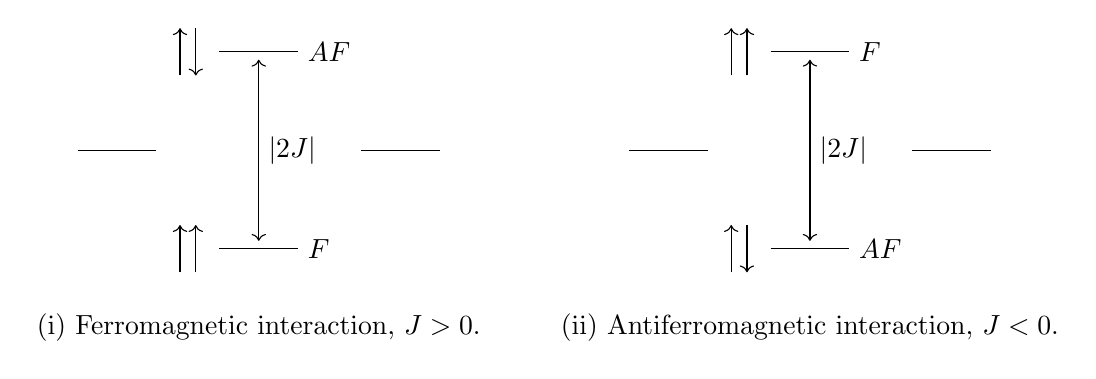
\begin{tikzpicture}
            \draw(0,0)--(1,0)node[right]{\(F\)};
            \draw(0,2.5)--(1,2.5)node[right]{\(AF\)};
            \draw[<->] (0.5,0.1)--node[right]{\(\abs{2J}\)}(0.5,2.4);
            \draw[->] (-0.5,-0.3)--(-0.5,0.3);
            \draw[->] (-0.3,-0.3)--(-0.3,0.3);
            \draw[->] (-0.5,2.2)--(-0.5,2.8);
            \draw[<-] (-0.3,2.2)--(-0.3,2.8);
            \draw (-1.8,1.25)--(-0.8,1.25);
            \draw (1.8,1.25)--(2.8,1.25);
            \node at (0.5,-1) {(i) Ferromagnetic interaction, \(J>0\).};

            \begin{scope}[shift={(7,0)}]
                \draw(0,0)--(1,0)node[right]{\(AF\)};
                \draw(0,2.5)--(1,2.5)node[right]{\(F\)};
                \draw[<->] (0.5,0.1)--node[right]{\(\abs{2J}\)}(0.5,2.4);
                \draw[->] (-0.5,-0.3)--(-0.5,0.3);
                \draw[<-] (-0.3,-0.3)--(-0.3,0.3);
                \draw[->] (-0.5,2.2)--(-0.5,2.8);
                \draw[->] (-0.3,2.2)--(-0.3,2.8);
                \draw (-1.8,1.25)--(-0.8,1.25);
                \draw (1.8,1.25)--(2.8,1.25);
                \node at (0.5,-1) {(ii) Antiferromagnetic interaction, \(J<0\).};
            \end{scope}
        \end{tikzpicture}
    \end{figure}
    
    We define the energy difference between the antiferromagnetic alignment and the ferromagnetic alignment states to be \(2J\),
    \begin{equation}
        2J = E_{\text{AF}}-E_{\text{F}}\,,
    \end{equation}
    where \(J\) is called the \textit{exchange parameter}. Then a ferromagnetic interaction has \(J>0\) while an antiferromagnetic interaction has \(J<0\).

    We've established that the main source of magnetism in ions comes from unpaired electrons, and hence the atomic orbitals with unpaired electrons are called \textit{magnetic orbitals}. How these magnetic orbitals interact determines whether the magnetic moments are coupled in a ferromagnetic or an antiferromagnetic way.

    \subsubsection{Heitler--London Model (Non-examinable)}
    The following discussion assumes familiarity of the contents in Part II A4: \textit{Theoretical Techniques}.

    Suppose we have two localised magnetic orbitals on two neighbouring ions, \(\phi_a(\vb{r})\) and \(\phi_b(\vb{r})\), each with an unpaired electron. Now we bring the two ions into proximity, so the electrons interact with the total Hamiltonian
    \begin{equation}
        \hat{H}=\hat{h}(1)+\hat{h}(2)+\frac{1}{r_{12}}
    \end{equation}
    in atomic units, where \(\hat{h}\) is the one-electron Hamiltonian. The Heitler--London model assumes the singlet (spin-antiparallel) and triplet (spin-parallel) states of the combined system to have spatial wavefunction
    \begin{align}
        \Phi_S & = \frac{\phi_a(1)\phi_b(2)+\phi_b(1)\phi_a(2)}{\sqrt{2(1+S^2)}} \\
        \Phi_T & = \frac{\phi_a(1)\phi_b(2)-\phi_b(1)\phi_a(2)}{\sqrt{2(1-S^2)}}\,,
    \end{align}
    combined with the triplet and singlet spin wavefunctions, respectively. Through some tedious algebra, the energies of the two states can be found to be
    \begin{align}
        E_S &= \expval{\hat{H}}{\Phi_S}=\frac{h_{aa}+2Sh_{ab}+h_{bb}+J+K}{1+S^2} \\
        E_T &= \expval{\hat{H}}{\Phi_T}=\frac{h_{aa}-2Sh_{ab}+h_{bb}+J-K}{1-S^2} \,,
    \end{align}
    where \(J\) is the coulomb integral and \(K\) is the exchange integral. The energy difference between the two states, expanded to order \(S^2\), is
    \begin{equation}
        E_S - E_T \approx 2K + 4Sh_{ab}\,.
    \end{equation}
    The resonance integral \(h_{ab}\) is negative, so it is common to define the \textit{hopping integral} \(t=-h_{ab}\) so that \(t\) is positive. We can recognise that the spin-antiparallel singlet state is exactly the antiferromagnetic state, and the spin-parallel triplet state is the ferromagnetic state, so we have
    \begin{equation}
        E_{\text{AF}}-E_{\text{F}}\approx2K-4St\,.
    \end{equation}
    It is conventional to write the spin coupling Hamiltonian to be \(\hat{H}=-2J\hat{\vb{S}}_1\vdot\hat{\vb{S}}_2\), and so this energy gap is \(2J\). Therefore we have
    \begin{equation}
        2J=2K-4St\,.
    \end{equation}
    Now both \(2K\) and \(4St\) are positive. The \(2K\) term comes from the exchange interaction between parallel spins, so when this term dominates, the system favours ferromagnetic alignment. This is sometimes known as the \textit{potential exchange term}. The \(4St\) terms arises from the electrons' ability to ``hop'' between atoms, which is only allowed if the electrons carry opposite spin (by Pauli exclusion principle). This leads to a reduction of the electrons' kinetic energy, and hence the system favours antiferromagnetic alignment if this term dominates. This is known as the \textit{kinetic exchange term}.

    \subsection{Direct Exchange}
    The above formula
    \begin{equation}
        2J=2K-4St
    \end{equation}
    applies when the two magnetic orbitals are close to each other so that both the exchange integral \(K\) and overlap integral \(S\) are non-negligible. This often requires the two ions to be \(\sim 4\ \text{\AA}\) apart or closer. This kind of interaction between unpaired spins by direct exchange interactions or electron hopping is known as \textit{direct exchange}. Usually, unless \(S\) in negligible for some reason (e.g. \(S=0\) due to symmetry), the kinetic term tends to dominate and the coupling tends to be antiferromagnetic.

    However, the metal ions in clusters are rarely close enough for these interactions to be significant, but still, communications between the spins are still clearly detected in many compounds. This suggests that there might be some indirect processes dominating the spin interactions in these species.

    \subsection{Superexchange}
    Superexchange is an indirect second order effect. It describes how two magnetic atoms that are far apart couple their spins through a non-magnetic atom, such as the ligand, that sits between them.
    
    Inheriting the nomenclature of the direct exchange, if a superexchange favours an antiferromagnetic state, then this is known as a kinetic superexchange, while if the ferromagnetic state is favoured, it is a potential superexchange. These are best illustrated with a few examples.

    \subsubsection{Potential Superexchange}
    Potential superexchange stabilises the ferromagnetic ground state through mutually orthogonal orbitals in the exchange pathway. This is comparatively rare, but can be achieved in several ways. The most common example is a pair of \(90^\circ\) orthogonal orbitals in \(\mathrm{M-X-M}\), where \(\mathrm{X}\) is a ligand.

    \begin{ex}
        \textit{\(90^\circ \) \(\mathrm{M}(e_g)-\mathrm{O}-\mathrm{M}(e_g)\) in \(\mathrm{[Cu(OH)_2Cu]^{2+}}\) dimer.}

        The two metal centres in the dimer are far apart, with little orbital overlap, so direct exchange is not possible.
        \begin{figure}[ht!]
            \centering
            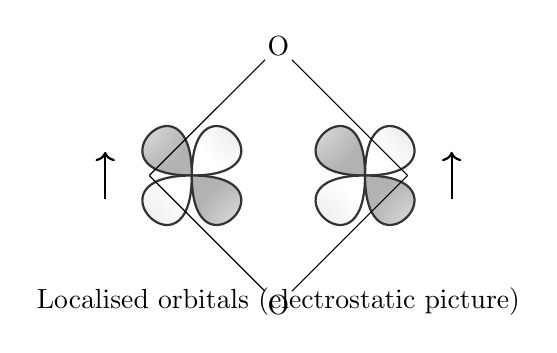
\begin{tikzpicture}
                \orbital[pos = {(-1.1,0)}, pcolor=white]{dyz};
                \orbital[pos = {(1.1,0)}, pcolor=white]{dyz};
                \node at (0,0){
                    \chemfig{[:45,2.2]O*4(--O--)}
                };
                \draw[thick,->] (-2.2,-0.3)--(-2.2,0.3);
                \draw[thick,->] (2.2,-0.3)--(2.2,0.3);

                \node at (0,-1.6) {Localised orbitals (electrostatic picture)};
            \end{tikzpicture}
        \end{figure}

        The bonding between metal and ligand is not purely ionic (crystal field approach), but instead has a significant covalent contribution. Thus the magnetic orbital on a metal may have some ligand character. Thus the ligand bears some spin density from both metals centres and acts as a mediator for communication between the spins formally located on metals the two centres.

        \begin{figure}[ht!]
            \centering
            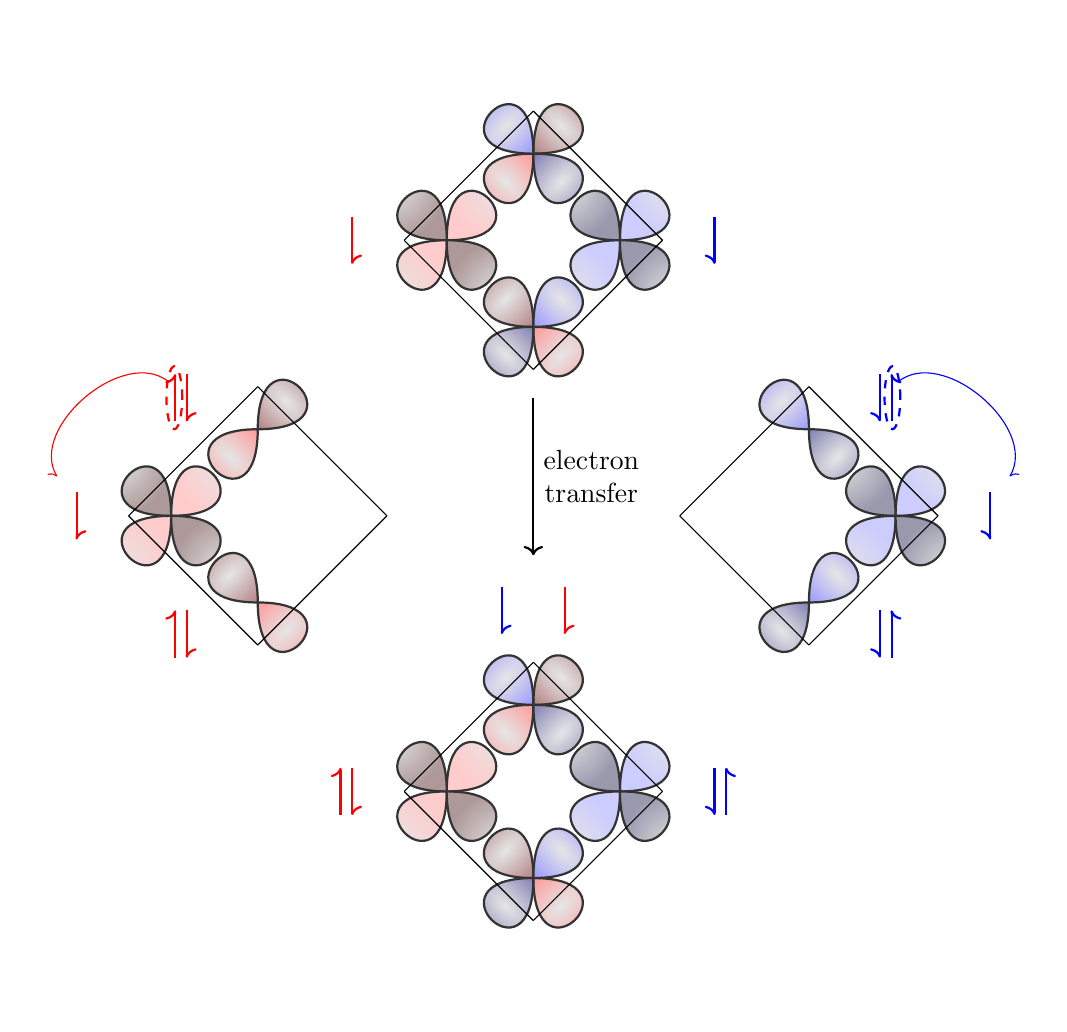
\begin{tikzpicture}
                \orbital[pos = {(-1.1,0)}, pcolor=red!20, ncolor=red!20!black!40]{dyz};
                \orbital[pos = {(1.1,0)}, pcolor=blue!20, ncolor=blue!20!black!40]{dyz};
                \node[rotate=225] at (0,1.1){\tikz{\orbital[pos = {(0,0)}, pcolor=red!40, ncolor=red!40!black!50]{py};}};
                \node[rotate=135] at (0,1.1){\tikz{\orbital[pos = {(0,0)}, pcolor=blue!40, ncolor=blue!40!black!50]{py};}};
                \node[rotate=315] at (0,-1.1){\tikz{\orbital[pos = {(0,0)}, pcolor=red!40, ncolor=red!40!black!50]{py};}};
                \node[rotate=45] at (0,-1.1){\tikz{\orbital[pos = {(0,0)}, pcolor=blue!40, ncolor=blue!40!black!50]{py};}};
                \node at (0,0){
                    \chemfig{[:45,2.2]*4(----)}
                };

                \draw[arrows = {->[left]},thick,red] (-2.3,0.3)--(-2.3,-0.3);
                \draw[arrows = {->[right]},thick,blue] (2.3,0.3)--(2.3,-0.3);

                \begin{scope}[shift={(-3.5,-3.5)}]
                    \orbital[pos = {(-1.1,0)}, pcolor=red!20, ncolor=red!20!black!40]{dyz};
                    \node[rotate=225] at (0,1.1){\tikz{\orbital[pos = {(0,0)}, pcolor=red!40, ncolor=red!40!black!50]{py};}};
                    \node[rotate=315] at (0,-1.1){\tikz{\orbital[pos = {(0,0)}, pcolor=red!40, ncolor=red!40!black!50]{py};}};
                    \node at (0,0){
                        \chemfig{[:45,2.2]*4(----)}
                    };
                    \draw[arrows = {->[left]},thick,red] (-2.3,0.3)--(-2.3,-0.3);
                    \draw[arrows = {->[left]},thick,red] (-0.9,1.8)--(-0.9,1.2);
                    \draw[arrows = {->[left]},thick,red] (-1.05,1.2)--(-1.05,1.8);
                    \draw[arrows = {->[left]},thick,red] (-0.9,-1.2)--(-0.9,-1.8);
                    \draw[arrows = {->[left]},thick,red] (-1.05,-1.8)--(-1.05,-1.2);
                    \draw[red,dashed,thick] (-1.06,1.5) ellipse (0.1 cm and 0.4 cm);
                    \draw[arrows = {->[right]},red] (-1.13,1.7) to[bend right=80] (-2.55,0.5);
                \end{scope}

                \begin{scope}[shift={(3.5,-3.5)}]
                    \orbital[pos = {(1.1,0)}, pcolor=blue!20, ncolor=blue!20!black!40]{dyz};
                    \node[rotate=135] at (0,1.1){\tikz{\orbital[pos = {(0,0)}, pcolor=blue!40, ncolor=blue!40!black!50]{py};}};
                    \node[rotate=45] at (0,-1.1){\tikz{\orbital[pos = {(0,0)}, pcolor=blue!40, ncolor=blue!40!black!50]{py};}};
                    \node at (0,0){
                        \chemfig{[:45,2.2]*4(----)}
                    };
                    \draw[arrows = {->[right]},thick,blue] (2.3,0.3)--(2.3,-0.3);
                    \draw[arrows = {->[right]},thick,blue] (0.9,1.8)--(0.9,1.2);
                    \draw[arrows = {->[right]},thick,blue] (1.05,1.2)--(1.05,1.8);
                    \draw[arrows = {->[right]},thick,blue] (0.9,-1.2)--(0.9,-1.8);
                    \draw[arrows = {->[right]},thick,blue] (1.05,-1.8)--(1.05,-1.2);
                    \draw[blue,dashed,thick] (1.06,1.5) ellipse (0.1 cm and 0.4 cm);
                    \draw[arrows = {->[left]},blue] (1.13,1.7) to[bend left=80] (2.55,0.5);
                \end{scope}

                \begin{scope}[shift={(0,-7)}]
                    \orbital[pos = {(-1.1,0)}, pcolor=red!20, ncolor=red!20!black!40]{dyz};
                    \orbital[pos = {(1.1,0)}, pcolor=blue!20, ncolor=blue!20!black!40]{dyz};
                    \node[rotate=225] at (0,1.1){\tikz{\orbital[pos = {(0,0)}, pcolor=red!40, ncolor=red!40!black!50]{py};}};
                    \node[rotate=135] at (0,1.1){\tikz{\orbital[pos = {(0,0)}, pcolor=blue!40, ncolor=blue!40!black!50]{py};}};
                    \node[rotate=315] at (0,-1.1){\tikz{\orbital[pos = {(0,0)}, pcolor=red!40, ncolor=red!40!black!50]{py};}};
                    \node[rotate=45] at (0,-1.1){\tikz{\orbital[pos = {(0,0)}, pcolor=blue!40, ncolor=blue!40!black!50]{py};}};
                    \node at (0,0){
                        \chemfig{[:45,2.2]*4(----)}
                    };

                    \draw[arrows = {->[left]},thick,red] (-2.45,-0.3)--(-2.45,0.3);
                    \draw[arrows = {->[left]},thick,red] (-2.3,0.3)--(-2.3,-0.3);
                    \draw[arrows = {->[right]},thick,blue] (2.45,-0.3)--(2.45,0.3);
                    \draw[arrows = {->[right]},thick,blue] (2.3,0.3)--(2.3,-0.3);
                    \draw[arrows = {->[left]},thick,blue] (-0.4,2.6)--(-0.4,2);
                    \draw[arrows = {->[left]},thick,red] (0.4,2.6)--(0.4,2);
                \end{scope}

                \draw[->,thick] (0,-2)--node[right,align=center]{electron\\ transfer}(0,-4);
            \end{tikzpicture}
        \end{figure}

        Note that the orbitals of the metals and ligands are divided into two orthogonal subsets --- one labelled in red and the other in blue. A simultaneous electron hopping allows the unpaired spin density to transfer to the ligand orbitals, and now these spins are close enough to have significant exchange interaction \(K\). Note that since the two ligand orbitals are orthogonal, the \(4St\) term vanishes; this orthogonality is inherited from the orthogonality of the two metal \(\mathrm{d}_{x^2-y^2}\) orbitals. Therefore, a parallel pair of spins are favoured in these ligand orbitals, which in turn favours a parallel pair of spins in the metal magnetic orbitals.

        If the electrons originally in the two metal magnetic orbitals are antiparallel, then this type of electron hopping will result in an antiparallel pair of electron on oxygen, which is disfavoured by Hund's first rule. Therefore, this type of potential superexchange results in ferromagnetic interaction.
    \end{ex}

    \subsubsection{Kinetic Superexchange}
    Kinetic superexchange stabilises the antiferromagnetic ground state through overlap of two magnetic orbitals which share the same anion orbital i.e. there is a net bonding interaction between the two magnetic orbitals.
    \begin{ex}
        \textit{\(180^\circ \) \(\mathrm{M}(e_g)-\mathrm{O}-\mathrm{M}(e_g)\) interaction.}

        Suppose now we have two magnetic \(e_g\) orbitals, but this time connected directly by a bridging \(\mathrm{O^{2-}}\) at \(180^\circ\).

        \begin{figure}[ht!]
            \centering
            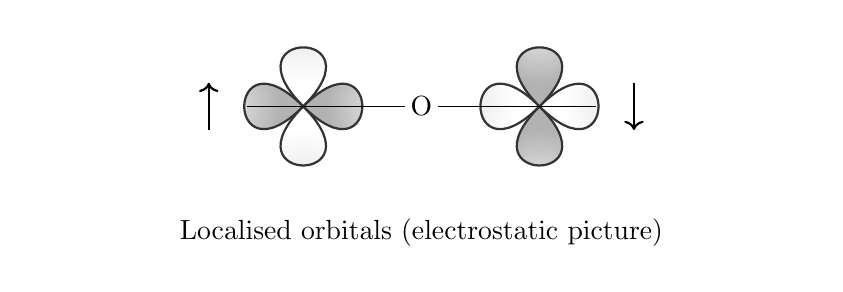
\begin{tikzpicture}
                \clip (-5,-2) rectangle (5,1);
                \node[rotate=45] at (-1.5,0){\tikz{\orbital[pos = {(0,0)}, pcolor=white]{dyz};}};
                \node[rotate=135] at (1.5,0){\tikz{\orbital[pos = {(0,0)}, pcolor=white]{dyz};}};
                \node at (0,0){
                    \chemfig{-[,2.1]O-[,2.1]}
                };
                \draw[thick,->] (-2.7,-0.3)--(-2.7,0.3);
                \draw[thick,->] (2.7,0.3)--(2.7,-0.3);

                \node at (0,-1.6) {Localised orbitals (electrostatic picture)};
                
            \end{tikzpicture}
        \end{figure}

        Again ligand-metal orbital interaction covalency enables electron transfers.
        \begin{figure}[ht!]
            \centering
            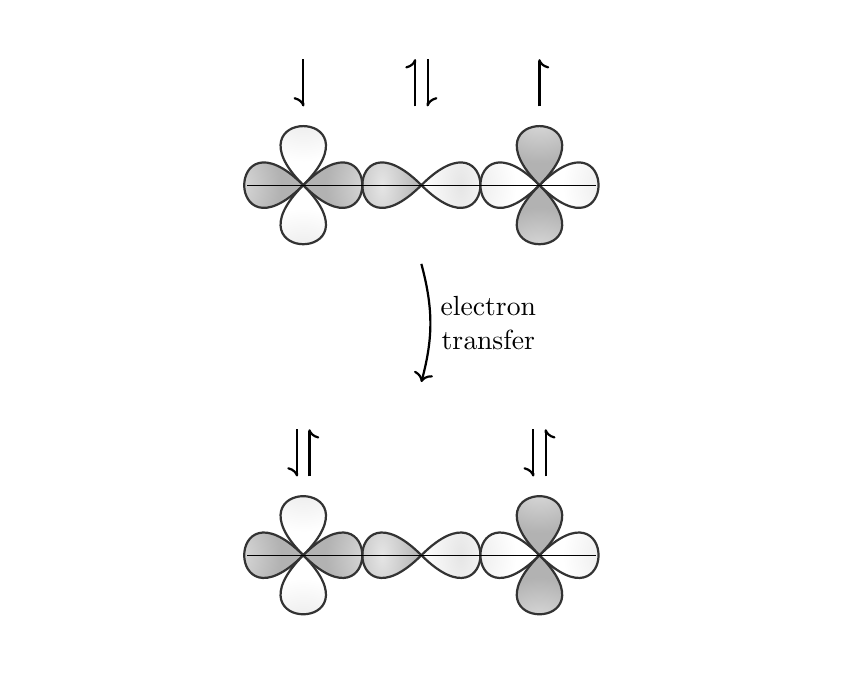
\begin{tikzpicture}
                \clip (-5,-6) rectangle (5,2);
                \node[rotate=45] at (-1.5,0){\tikz{\orbital[pos = {(0,0)}, pcolor=white]{dyz};}};
                \node[rotate=135] at (1.5,0){\tikz{\orbital[pos = {(0,0)}, pcolor=white]{dyz};}};
                \orbital[pos = {(0,0)}, pcolor=white]{py};
                \node at (0,0){
                    \chemfig{-[,2.1]-[,2.1]}
                };
                \draw[arrows = {->[right]},thick] (-1.5,1.6)--(-1.5,1);
                \draw[arrows = {->[right]},thick] (1.5,1)--(1.5,1.6);
                \draw[arrows = {->[left]},thick] (-0.08,1)--(-0.08,1.6);
                \draw[arrows = {->[left]},thick] (0.08,1.6)--(0.08,1);

                \draw[thick,->] (0,-1)to[bend left=15]node[right,align=center]{electron\\ transfer}(0,-2.5);

                \begin{scope}[shift={(0,-4.7)}]
                    \node[rotate=45] at (-1.5,0){\tikz{\orbital[pos = {(0,0)}, pcolor=white]{dyz};}};
                    \node[rotate=135] at (1.5,0){\tikz{\orbital[pos = {(0,0)}, pcolor=white]{dyz};}};
                    \orbital[pos = {(0,0)}, pcolor=white]{py};
                    \node at (0,0){
                        \chemfig{-[,2.1]-[,2.1]}
                    };
                    \draw[arrows = {->[right]},thick] (-1.58,1.6)--(-1.58,1);
                    \draw[arrows = {->[right]},thick] (1.58,1)--(1.58,1.6);
                    \draw[arrows = {->[right]},thick] (-1.42,1)--(-1.42,1.6);
                    \draw[arrows = {->[right]},thick] (1.42,1.6)--(1.42,1);
                \end{scope}
            \end{tikzpicture}
        \end{figure}

        This hopping stabilisation is only possible if the two magnetic orbitals of metals initially carries opposite spins, so it results in antiferromagnetic coupling.
    \end{ex}

    The example shown above is the \(\sigma\)-pathway of kinetic superexchange. A \(\pi\) pathway is also possible between two \(t_{2g}\) magnetic orbitals, with the arrangement shown in the figure below. This is usually weaker than the \(\sigma\) superexchange.
    \begin{figure}[ht!]
        \centering
        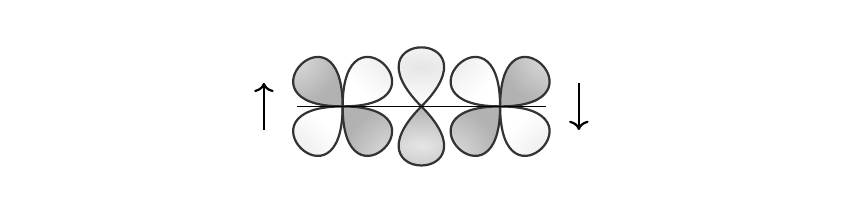
\begin{tikzpicture}
            \clip (-5,-1) rectangle (5,1);
            \node at (-1,0){\tikz{\orbital[pos = {(0,0)}, pcolor=white]{dyz};}};
            \node[rotate=90] at (1,0){\tikz{\orbital[pos = {(0,0)}, pcolor=white]{dyz};}};
            \orbital[pos = {(0,0)}, pcolor=white]{pz};
            \node at (0,0){
                \chemfig{-[,1.5]-[,1.5]}
            };
            \draw[thick,->] (-2,-0.3)--(-2,0.3);
            \draw[thick,->] (2,0.3)--(2,-0.3);
            
        \end{tikzpicture}
    \end{figure}

    \subsubsection{Angular Dependence of Superexchange}
    As for the direct exchange, kinetic superexchange tends to dominate over potential superexchange unless \(S\) is small e.g. due to symmetry. As a result, the coupling constant \(J\) tends to have strong angular dependence.

    \begin{ex}
        \textit{Planar copper dimers with two hydroxyl bridges.}

        We continue investigating the following family of planar copper dimers.

        \begin{figure}[ht!]
            \centering
            \begin{tikzpicture}
                \clip (-5,-2) rectangle (5,2);
                \node at (0,0){
                    \chemfig{[:135,1.5]Cu*4(-O(-[,0.9]H)-Cu(-[:135]@{a}N)(-[:-135]@{b}N)-O(-[,0.9]H)-)(-[:45]@{c}N)(-[:-45]@{d}N)}
                    \chemmove{\draw[-,thick,shorten <=0.5mm, shorten >=0.5mm](a)..controls +(-135:7mm) and +(135:7mm)..(b);}
                    \chemmove{\draw[-,thick,shorten <=0.5mm, shorten >=0.5mm](c)..controls +(-45:7mm) and +(45:7mm)..(d);}
                };
            \end{tikzpicture}
            
        \end{figure}

        By changing the size of the \(\mathrm{N-R-N}\) ligand, we can alter the \(\mathrm{Cu-O-Cu}\) bond angle \(\theta\). When \(\theta=90^\circ\) exactly, this is the kinetic superexchange example we met before. Since the two orbitals are orthogonal, kinetic exchange is not possible so \(J\) is positive (ferromagnetic). As the bond angle deviates from \(90^\circ\), kinetic superexchange becomes possible via scheme shown in the previous example. Hence \(J\) begins to decrease.

        \begin{figure}[ht!]
            \centering
            % This file was created with matplot2tikz v0.4.0.
\begin{tikzpicture}

\definecolor{darkgray176}{RGB}{176,176,176}
\definecolor{steelblue31119180}{RGB}{31,119,180}

\begin{axis}[
tick align=outside,
tick pos=left,
x grid style={darkgray176},
xlabel={\(\displaystyle \theta\) / \(\displaystyle ^\circ\)},
xmin=88.8, xmax=115.2,
xtick style={color=black},
y grid style={darkgray176},
ylabel={\(\displaystyle 2J\) / \(\displaystyle \mathrm{cm}^{-1}\)},
ymin=-1289.49752214157, ymax=642.670431028157,
ytick style={color=black}
]
\addplot [draw=steelblue31119180, fill=steelblue31119180, mark=x, only marks, mark size=3]
table{%
x  y
95.5402423714721 178.706130417728
96.5325245872582 107.547153049391
96.9184112744514 62.2640866893312
98.682469388128 -118.867882623477
100.308708845054 -193.261459915636
102.238147328028 -354.986570004093
102.541343830572 -409.97299194447
102.92723304127 -400.269488300437
104.002205441705 -500.539124664589
107.6681352788 -714.016204833318
109.928337023874 -869.272263137848
};
\addplot [semithick, black]
table {%
90 554.844614974987
96 115.715534709139
102 -323.413545556708
108 -762.542625822556
114 -1201.6717060884
};
\end{axis}

\end{tikzpicture}

            \caption{The exchange parameter against ligand-metal bond angle for copper dimer.}
            \label{Fig:ligand_J}
        \end{figure}

        The \(J\) against \(\theta\) is plotted in \cref{Fig:ligand_J} for a range of compounds. It is found that the data shows a very good linearity against \(\theta\), with the empirical relationship
        \begin{equation}
            2J=(-74\theta + 7215)\unit{cm}^{-1}
        \end{equation}
        for \(\theta\ge 90^\circ\) measured in degrees. Since the kinetic superexchange is much stronger than potential superexchange, we only need very small spatial overlap (via ligand) for the kinetic term to dominate --- in this case \(J=0\) when \(\theta=97.5\).
    \end{ex}

    From the above example, it can be seen that the ferromagnetic coupling is fragile. The potential superexchange can be easily overwhelmed by the kinetic superexchange even with only a tiny amount of spatial overlap. It seems that it is therefore very difficult to produce ferromagnetic materials like magnets --- and even if we can make one by carefully controlling the geometry of orbital interaction, the small \(\abs{J}\) makes the ferromagnetic alignment easily scrambled by thermal activation once \(k_B T\approx \abs{J}\) at room temperatures.

    We will see how this problem is resolved when we have a magnetic network.

    \subsubsection{General Features of Superexchange}
    To conclude:
    \begin{itemize}
        \item The kinetic exchange pathways are usually stronger than potential superexchange. As a consequence, when competing pathways are present the resultant interaction tends to be antiferromagnetic. Exceptions occur when all superexchange pathways involve orthogonal orbitals so that kinetic exchange is not possible.
        \item Because of the better overlap in \(\sigma\)-bonds, the \(\sigma\)-type superexchange tends to be greater than \(\pi\)-superexchange, i.e. the interactions involving the \(e_g\) orbitals tend to predominate. 
        \item The magnitude of \(J\) is very sensitive to overlap (covalency). As a consequence \(\abs{J}\) tends to increase as we move from left to right (better energy match with ligand) or move down the group (more diffuse orbitals), and for softer and more polarisable ligands.
        \item For ions with more than one magnetic orbitals, both \(\sigma\) and \(\pi\) type interactions are possible.
    \end{itemize}

    \subsection{Magnetic Susceptibility of Clusters}
    Magnetic coupling makes the susceptibility of clusters deviate from the simple Curie law --- and the resulting general expression of \(\chi\) is usually quite complicated: coupling splits the system to a number of energy levels, with population given by the Boltzmann distribution, and each contributes accordingly to the total magnetic susceptibility. We will first investigate the high temperature and low temperature limits, which are quite easy to work out, before discussing how to find the general expression of \(\chi(T)\) for a cluster.

    \subsubsection{High Temperature Limit}
    If the temperature is high enough with \(k_B T\gg \abs{J}\), we can simply ignore the coupling and act as if the spin carriers are non-interacting. If the cluster carries spins \(\{S_1,\dots,S_n\}\), the molar susceptibility of the cluster is therefore the sum of the molar susceptibility of the individual spin carriers in the ideal Curie case,
    \begin{equation}
        \chi T=\sum_{i=1}^{n}\frac{N_A g^2 \mu_{\text{B}}^2}{3k_B} S_i (S_i+1)\,.
    \end{equation}
    If we use \(g\approx 2.0\), this gives
    \begin{equation}
        \chi T\approx\sum_{i=1}^{n}\frac{1}{2}S_i (S_i+1)\unit{emu}\unit{K}\unit{mol}^{-1}
    \end{equation}
    in cgs units.

    \subsubsection{Low Temperature Limit}
    Now, if \(k_B T\ll\abs{J}\), only the overall magnetic ground state is occupied. The whole cluster acts as like a single spin carrier with total spin \(S_{\text{T}}\), so that
    \begin{equation}
        \chi T=\frac{N_A g^2 \mu_{\text{B}}^2}{3k_B} S_{\text{T}} (S_{\text{T}}+1)\approx \frac{1}{2}S_{\text{T}}(S_{\text{T}}+1)\unit{emu}\unit{K}\unit{mol}^{-1}\,.
    \end{equation}
    Note that to use Curie law, we must have \(\frac{H}{T} / k_B\mu_{\text{B}}^{-1}\ll 1\) so that we are in the linear region of Brillouin's function. Since we take \(T\) to be small, \(H\) needs to small as well.


    The total spin \(S_{\text{T}}\) for the magnetic ground state varies from case to case. If all the coupling within the cluster is ferromagnetic, the magnetic ground state clearly has all spins aligned so
    \begin{equation}
        S_{\text{T}}=\sum_{i=1}^{n}S_i\,.
    \end{equation}
    If we have a chain of \(n\) identical spins \(S\), then the magnetic ground state has the spins alternating in direction. If \(n\) is even, then the ground states have all spins cancelled out so \(S_{\text{T}}=0\), and hence
    \begin{equation}
        \chi T =0\,.
    \end{equation}
    If \(n\) is odd, then we have all spins cancelled except one spin left out so \(S_{\text{T}}=S\) and
    \begin{equation}
        \chi T=\frac{N_A g^2 \mu_{\text{B}}^2}{3k_B} S(S+1)\,.
    \end{equation}
    If the coupling geometry is any more complex, then we need to find ground state \(S_{\text{T}}\) \textit{ad hoc}.

        
    


    

    

    
    



    \newpage
    \part*{Appendices}
    \addcontentsline{toc}{part}{\protect\numberline{}Appendices}
    \appendix
\end{document}